 %  LaTeX support: latex@mdpi.com 
%  For support, please attach all files needed for compiling as well as the log file, and specify your operating system, LaTeX version, and LaTeX editor.

%=================================================================
\documentclass[risks,article,submit,pdftex,moreauthors]{Definitions/mdpi} 

%=================================================================
% MDPI internal commands - do not modify
\firstpage{1} 
\makeatletter 
\setcounter{page}{\@firstpage} 
\makeatother
\pubvolume{1}
\issuenum{1}
\articlenumber{0}
\pubyear{2025}
\copyrightyear{2025}
\datereceived{---} 
\daterevised{---} 
\dateaccepted{---} 
\datepublished{---} 
\hreflink{https://doi.org/} 

%=================================================================
% Add packages and commands here
% Custom commands from dissertation
\newcommand{\E}{\mathbb{E}}
\newcommand{\supprepo}{\href{https://github.com/AbdullahHassan176/NFGARCH}{https://github.com/AbdullahHassan176/NFGARCH}}
\newcommand{\tablesdir}{results/dissertation_tables/}
\newcommand{\roth}[1]{\rotatebox[origin=c]{60}{\makecell{#1}}}

% Additional packages for custom commands
\usepackage{makecell} % For \makecell command used in
%\usepackage{amsmath, amssymb, amsfonts} 
\usepackage{float}                   
%\usepackage{graphicx}
%\usepackage[T1]{fontenc}
%\usepackage{bm}
%\usepackage[english]{babel}
%\usepackage{booktabs}
%\usepackage{amsthm}
%\usepackage[titletoc]{appendix}
%\usepackage{mathrsfs}
%\usepackage{fancyhdr}
%\usepackage{multirow}
%\usepackage{tikz}
%\usepackage{xcolor}
%\usepackage{tabularx}   
%\usepackage{makecell}
%\usepackage{siunitx} 
%\usepackage{pdflscape}  
%\usepackage{rotating}  
%\usepackage{array}  
\usepackage{graphicx}
\usepackage{array}
\usepackage{tikz}
\usetikzlibrary{arrows.meta, positioning}

\setlength{\parindent}{12pt}\setlength{\parskip}{0pt}
\renewcommand{\sectionmark}[1]{\markright{\thesection\ #1}}
\fancyhf{}
\fancyhead[RO]{\bfseries\thepage}
\fancyhead[LO]{\bfseries\rightmark}
\renewcommand{\headrulewidth}{0.5pt}
\renewcommand{\footrulewidth}{0pt}
\addtolength{\headheight}{0.5pt}
\sloppy                     
\emergencystretch=2em         
\tolerance=1000            
\hbadness=10000 

\fancypagestyle{plain}{%
  \fancyhf{}
  \renewcommand{\headrulewidth}{0pt}
}
%\usepackage{listings}
%\lstset{
%    language=R,
%    basicstyle=\scriptsize\ttfamily,
%    commentstyle=\ttfamily\color{green},
 %   numbers=left,
 %   numberstyle=\ttfamily\color{white}\footnotesize,
%    stepnumber=1,
 %   numbersep=5pt,
 %   backgroundcolor=\color{white},
 %   showspaces=false,
 %   showstringspaces=false,
 %   showtabs=false,
 %   frame=single,
 %   tabsize=2,
 %   captionpos=b,
  %  breaklines=true,
  %  breakatwhitespace=false,
  %  title=\lstname,
 %   escapeinside={},
 %   keywordstyle={},
 %   morekeywords={}
%    }
%\usepackage{hyperref}
%\hypersetup{
 %   hidelinks,
 %   pdfpagelayout=OneColumn  % optional
%}
% Note: \rotatebox is provided by graphicx package (already loaded by mdpi.cls)

% Numeric alignment defaults
%\usepackage{siunitx}
%\sisetup{
%  detect-all,
%  table-align-text-post = false,
%  input-symbols = (),
 % table-number-alignment = center
%}

% Graphics path (updated for Overleaf structure)
\graphicspath{{./}{./results/}{./results/figures/}}

%=================================================================
% Full title of the paper (Capitalized)
\Title{Normalising Flow Enhanced GARCH Models: A Two-Stage Framework for Flexible Innovation Modelling in Financial Time Series}

% MDPI internal command: Title for citation in the left column
\TitleCitation{Normalising Flow Enhanced GARCH Models: A Two-Stage Framework for Flexible Innovation Modelling in Financial Time Series}

% Author Orchid ID: enter ID or remove command
%\newcommand{\orcidauthorA}{0000-0000-0000-000X}
\newcommand{\orcidauthorB}{0000-0003-4091-1901}
\newcommand{\orcidauthorC}{0000-0003-2832-3584}

% Authors, for the paper (add full first names)
\Author{Abdullah Hassan $^{1}$, Farai Mlambo $^{2}$\orcidB{} and Wilson Tsakane Mongwe $^{1,*}$\orcidC{}}

% MDPI internal command: Authors, for metadata in PDF
\AuthorNames{Abdullah Hassan, Farai Mlambo and Wilson Tsakane Mongwe}

% MDPI internal command: Authors, for citation in the left column (Chicago style for Risks journal)
\AuthorCitation{Hassan, Abdullah, Farai Mlambo, and Wilson Tsakane Mongwe.}

% Affiliations / Addresses
\address{%
$^{1}$ \quad School of Statistics and Actuarial Science, University of the Witwatersrand, Johannesburg, South Africa\\
$^{2}$ \quad Graduate School of Business Administration, University of the Witwatersrand, Johannesburg, South Africa\\
$^{*}$ \quad Correspondence: wilsonmongwe@gmail.com
}


% Abstract (Do not insert blank lines, i.e. \\) 
\abstract{ We introduce the Normalising Flow GARCH (NF-GARCH), a two-stage hybrid framework that enhances traditional GARCH models by replacing restrictive parametric innovation distributions with learned densities via Normalising Flows. Our approach preserves the interpretability of standard variance dynamics while addressing the common issue of innovation misspecification. In the first stage, we estimate standard GARCH variants (sGARCH, TGARCH, and gjrGARCH) to extract standardised residuals. In the second stage, a Masked Autoregressive Flow learns the underlying residual distribution, with samples from the flow subsequently driving the GARCH recursion for out-of-sample forecasting. Evaluated on 13 daily financial series (six FX pairs and seven equities), NF-GARCH demonstrates systematic, statistically significant improvements in forecast accuracy for skewed-$t$ baselines. Wilcoxon signed-rank tests confirm superior performance specifically for gjrGARCH-sstd and sGARCH-sstd specifications. While the framework offers enhanced flexibility and generative realism, we observe that computational overhead is increased, and the log-variance specification of eGARCH exhibits instability when paired with flow-based innovations. These results suggest that while NF-GARCH effectively captures empirical tail behavior in univariate settings, future research should explore conditional flow architectures and multivariate extensions to account for time-varying innovation shapes. For risk management, gains are most relevant where skewed-$t$ baselines are used and where closer residual realism supports scenario analysis; effect sizes remain modest relative to model risk and implementation cost.}

% Keywords
\keyword{Normalising Flows; GARCH; Volatility; Financial Time Series; Heavy Tails; Financial Econometrics; Stylized Facts} 

%%%%%%%%%%%%%%%%%%%%%%%%%%%%%%%%%%%%%%%%%%
\begin{document}

%%%%%%%%%%%%%%%%%%%%%%%%%%%%%%%%%%%%%%%%%%
\section{Introduction}

Empirical analysis over the past two decades has shown that financial returns exhibit clustering, where similarly large movements often follow large movements \citep{cont2001empirical, aloud2013stylized}. These returns further exhibit heavy tails and asymmetric responses, with negative shocks increasing volatility more than positive shocks \citep{cont2001empirical}. Generalized Autoregressive Conditional Heteroskedasticity (GARCH) models address clustering through autoregressive variance dynamics \citep{bollerslev1986generalised}. However, their innovation distributions are typically limited to Gaussian or Student-$t$ forms. This limitation fails to capture the skewness and tail behaviour that are critical for risk assessment.

The choice of innovation distribution in GARCH models has long been recognized as critical to forecasting accuracy \citep{bollerslev1987conditionally, ederington2005forecasting}. Early specifications assumed Gaussian innovations, but this was quickly challenged by evidence of heavy tails \citep{bollerslev1986generalised}. \cite{bollerslev1987conditionally} introduced Student-$t$ innovations to capture excess kurtosis. \cite{hansen1994autoregressive} demonstrated that even small innovation misspecifications propagate into substantial forecast errors. Despite advances with skewed distributions, parametric approaches impose restrictive functional forms \citep{fernandez1998multivariate}.

Semi-parametric alternatives include kernel-based density estimation and nonparametric conditional density methods, though these suffer from curse-of-dimensionality issues and sensitivity to bandwidth choice \citep{engle1993measuring, hansen2004nonparametric, silverman1986density}. Machine learning approaches have also been explored to enhance innovation modelling. Examples include Long Short-Term Memory networks integrated with GARCH, which can improve forecasting but sacrifice interpretability due to the black-box nature of neural network methods \citep{kim2018forecasting, hossain2008comparison}. In regulated financial applications, interpretability and testable statistical properties remain important \citep{harvey2022machine, rudin2019stop}.

Normalising Flows represent a robust framework for constructing intricate probability distributions by applying a series of invertible transformations \citep{rezende2015variational, mongwe2025bayesian}. The initial probability density undergoes a sequence of mappings by systematically employing the change of variables formula, yielding a tractable complex distribution. Normalising Flows have the potential to address limitations of both parametric and alternative approaches to modelling innovations by providing exact likelihood evaluation through invertible transformations \citep{rezende2015variational, papamakarios2021normalising, seitz2022garchnf}. Despite extensive research, limited empirical evidence exists on whether flexible, nonparametric innovation distributions, specifically those learned via Normalising Flows, provide systematic improvements when integrated into classical GARCH frameworks without modifying the volatility recursion. This gap motivates a two-stage modular approach that we introduce in this paper.

\textbf{Research gap and contributions.} Semi-parametric and kernel-based GARCH specifications \citep{engle1993measuring, hansen2004nonparametric} relax the innovation law but differ in implementation, bandwidth demands, and scalability. Joint (end-to-end) flow--GARCH estimation \citep{seitz2022garchnf} entangles volatility and innovation learning, making it difficult to attribute forecast improvements to either component. We target the distinct question: if the volatility recursion is held fixed and estimated as in standard practice, does replacing the parametric residual law with a normalising flow improve forecasts and residual realism? Our specific contributions are: (i) a modular two-stage NF-GARCH design that preserves classical variance dynamics while learning a flexible innovation density; (ii) systematic evaluation on thirteen daily FX and equity series using out-of-sample metrics, Wilcoxon tests, distributional distances, VaR backtesting, and stress windows; (iii) empirical evidence that gains concentrate on skewed-$t$ baselines (gjrGARCH-sstd, sGARCH-sstd) rather than Gaussian baselines, consistent with the hypothesis that flow-based density learning addresses residual skewness that parametric forms miss; (iv) demonstration that eGARCH instability under flow augmentation arises from parameter redundancy between the log-variance recursion and the flow's skewness modelling; (v) a practical characterization of when NF-GARCH should be preferred over standard GARCH in risk management contexts.

We propose Normalising Flow-GARCH (NF-GARCH), a hybrid approach that keeps the standard GARCH variance recursion but replaces parametric residuals with a nonparametric learned Normalising Flow. The innovation distribution can match empirical characteristics better without losing interpretability in the variance process. We evaluate four GARCH variants (sGARCH, TGARCH, GJR-GARCH, eGARCH) and their NF-augmented versions on 13 daily financial series (six FX pairs, seven equities) using chronological splits and time-series cross-validation. Metrics include out-of-sample loss (MSE, MAE), distributional distances, and VaR calibration.


The method works in two stages. First, fit standard GARCH models and extract standardised residuals. Second, train a Normalising Flow on these residuals, then use flow samples to drive the original GARCH recursion. This preserves the traditional volatility structure and allows modular estimation. The flow's shape stays state-invariant—it scales with $\sigma_t$ but doesn't depend on it. An extension of this work is end-to-end designs that jointly optimize flow and GARCH parameters. We avoid the end-to-end integration of GARCH and normalising flows in this work for interpretability and parameter identifiability, and leave this as an aspect we will explore in future work. 

The remainder of this paper is structured as follows: We first present the background to volatility modelling, Normalising flows and our two stage hybrid approach in Section \ref{sec:background}, we then present the experiment setup we use in Section \ref{sec:experiments}. We present the results and discussion in Section \ref{sec:results} and finally conclude in Section \ref{sec:conclusion}.

%%%%%%%%%%%%%%%%%%%%%%%%%%%%%%%%%%%%%%%%%%
\section{Background}
\label{sec:background}
%%%%%%%%%%%%%%%%%%%%%%%%%%%%%%%%%%%%%%%%%%%%%%%%%%%%%%%%%%%%%%%%%%%%%%%%%%%%%%
% Theoretical Review - ARCH and GARCH Modelling

\subsection{Volatility modelling}

The foundation of standard Autoregressive Moving Average (ARMA) analysis relies on the assumption that the mean and unconditional variance of the time series remain constant over time, implying stationarity \citep{BoxJenkins1976, pankratz1991forecasting}. Techniques such as plotting the Autocorrelation Function (ACF) and Partial Autocorrelation Function (PACF), alongside tests like the Augmented Dickey-Fuller (ADF) test, are employed to ascertain stationarity. For non-stationary time series, transformations are applied to achieve stationarity, as detailed by \cite{pankratz1991forecasting}.

In addressing the challenge of high volatility in forecasting financial time series, recent developments have led to adopting models like Generalized Autoregressive Conditional Heteroskedasticity (GARCH) models. In GARCH processes, volatility (i.e., the variance of disturbances) is explicitly modeled. Tests for stationarity and other diagnostics closely parallel those used in ARMA analysis. Asymmetric extensions such as EGARCH \citep{nelson1991conditional}, TGARCH \citep{zakoian1994threshold}, and GJR-GARCH \citep{glosten1993relation} allow negative shocks to affect volatility differently from positive ones, capturing the leverage effect documented in equity and FX returns \citep{black1976studies, christie1982stochastic, cont2001empirical}.

\cite{engle1982autoregressive} showed that the serial correlation in squared returns, or conditional heteroskedasticity, can be modelled using an autoregressive conditional heteroskedasticity (ARCH) model of the form:
\begin{equation}
Y_t = \E_{t-1}[Y_t] + \epsilon_t
\end{equation}
\begin{equation}
\epsilon_t = \sigma_t z_t
\end{equation}
\begin{equation}
\sigma_t^2 = a_0 + a_1 \epsilon_{t-1}^2 + a_2 \epsilon_{t-2}^2 + \dots + a_q \epsilon_{t-q}^2  
\end{equation}
where \(\E_{t-1}[\cdot]\) represents the conditional expectation on all information that is available at time \(t-1\) and \(\epsilon_t\) is modelled as the product of a standardised shock \(z_t\) and time-varying volatility \(\sigma_t\) such that \(z_t\) is a sequence of independent and identically distributed ("iid") random variables with mean zero and unit variance. In the ARCH model, \(z_t\) is assumed to be independent and identically distributed with a standard normal distribution. The restrictions \(a_0 > 0\) and \(a_i >= 0\) \(i = 1,..,q\) are required for \(\sigma_t^2 > 0\).\\

An important extension of the ARCH model proposed by \cite{bollerslev1986generalised} replaces the AR (p) representation with an ARMA (p,q) formulation:

\begin{equation}
\sigma_t^2 = a_0 + \sum_{j=1}^p b_j \sigma_{t-j}^2 + \sum_{i=1}^q a_i \epsilon_{t-i}^2, 
\end{equation}
where the coefficients \(a_i\) \((i=0,..,q)\) and \(b_j\) \((j=1,..,p)\) are all assumed to be positive to ensure that the conditional variance \(\sigma_t^2\) is always positive. The model in (2.4) together with (2.1) - (2.2) is known as the generalised ARCH or GARCH (p,q) model. When \(p=0\), the GARCH model reduces to the ARCH model.


%%%%%%%%%%%%%%%%%%%%%%%%%%%%%%%%%%%%%%%%%%%%%%%%%%%%%%%%%%%%%%%%%%%%%%%%%%%%%%
% Theoretical Review - Normalising Flows

\subsection{Normalising Flows}

Normalising Flows represent a robust framework for constructing intricate probability distributions by applying a series of invertible transformations \citep{rezende2015variational, mongwe2025analyzing}. The initial probability density undergoes a sequence of mappings by systematically employing the change of variables formula, yielding a tractable complex distribution. The term Normalising Flow aptly describes this process, as the density effectively "flows" through the sequence of transformations, culminating in a normalised probability distribution \citep{rezende2015variational}.

Based on the initial framework developed by \cite{rezende2015variational}, we consider a finite sequence of transformations where each mapping is invertible and smooth. If we let \( f \) denote such a mapping with its corresponding inverse \( f^{-1} \), then for a random variable \(\mathbf{X}\) with an initial density \( p_\mathbf{X}(\mathbf{x}) \), the transformed random variable \(\mathbf{Y} = f(\mathbf{X})\) follows a density:
\begin{equation}
p_\mathbf{Y}(\mathbf{y}) = p_\mathbf{X}\left(f^{-1}(\mathbf{y})\right) \left|\det \frac{\partial f^{-1}(\mathbf{y})}{\partial \mathbf{y}}\right|
\end{equation}


This relationship is derived by invoking the inverse function theorem, which governs the behaviour of Jacobians for invertible functions. By composing multiple such mappings, one can generate arbitrarily complex densities. Specifically, if a random variable \(\mathbf{X}\) with density \(p_\mathbf{X}(\mathbf{x})\) is subjected to a sequence of \(K\) transformations \(f_1, f_2, \dots, f_K\), the resulting density of the final variable \(\mathbf{Z}_K = f_K \circ \cdots \circ f_1(\mathbf{X})\) can be written in terms of the base variable and the Jacobians of the forward maps: \(p_{\mathbf{Z}_K}(\mathbf{z}_K) = p_\mathbf{X}(\mathbf{x}_0) \prod_{k=1}^{K} \left|\det J_{f_k}(\mathbf{z}_{k-1})\right|^{-1}\), where \(\mathbf{z}_0 = \mathbf{x}_0\) and \(J_{f_k}\) denotes the Jacobian of \(f_k\). Equivalently, in inverse form,
\begin{equation}
p_{\mathbf{Z}_K}(\mathbf{z}_K) = p_\mathbf{X}(\mathbf{x}) \prod_{k=1}^{K} \left|\det \frac{\partial f_k^{-1}(\mathbf{z}_k)}{\partial \mathbf{z}_k}\right|
\end{equation}


As suggested by \cite{kobyzev2020normalising}, the trajectory traced by the sequence of transformed random variables \(\mathbf{Z}_k\), starting from the initial distribution \(p_\mathbf{X}(\mathbf{x})\), constitutes the flow. In contrast, the sequence of intermediate densities \(p_{\mathbf{Z}_k}(\mathbf{z}_k)\) defines the Normalising Flow.\\

%%%%%%%%%%%%%%%%%%%%%%%%%%%%%%%%%%%%%%%%%%%%%%%%%%%%%%%%%%%%%%%%%%%%%%%%%%%%%%
% Theoretical Review - Normalising Flows in GARCH Residuals (NF-GARCH)

\subsection{Normalising Flows in GARCH Residuals (NF-GARCH)}
\noindent 
Traditional GARCH-type models, including sGARCH, EGARCH, and TGARCH, often assume that the residuals \( z_t \) follow a known parametric distribution such as Gaussian, Student-\( t \), or Generalised Error Distribution. However, empirical studies have shown that these fixed-distribution assumptions are often too restrictive to capture the true nature of financial return innovations, which can be skewed, heavy-tailed, or even multi-modal. The choice of innovation distribution is critical for tail-sensitive risk measures such as Value-at-Risk and Expected Shortfall \citep{hansen1994autoregressive, bauwens2006multivariate}.

To address this, we replace the assumption \( z_t \sim \mathcal{N}(0,1) \) with:
\[
z_t = f(u_t), \quad u_t \sim \mathcal{N}(0, I_d)
\]
where \( f: \mathbb{R}^d \rightarrow \mathbb{R}^d \) is a sequence of invertible, differentiable transformations—i.e., a Normalising Flow. This transforms a simple base distribution (such as standard normal) into a rich, learned distribution for residuals \( z_t \), thereby enabling greater flexibility in capturing empirical data characteristics. While alternative heavy-tailed base distributions such as the Student-t could be considered for the base distribution, we adopt a standard normal base for tractability and comparability, with tail flexibility introduced through the learned flow transformations.

Given a base density \( p_U(u) \) and an invertible transformation \( z = f(u) \), the transformed density of \( z \) is given by the change-of-variables formula:
\[
p_Z(z) = p_U(f^{-1}(z)) \left| \det \left( \frac{\partial f^{-1}(z)}{\partial z} \right) \right|
\]
or, equivalently:
\[
\log p_Z(z) = \log p_U(u) - \sum_{i=1}^K \log \left| \det \left( \frac{\partial f_i}{\partial h_{i-1}} \right) \right|
\]
where \( f = f_K \circ \cdots \circ f_1 \), and \( h_i = f_i(h_{i-1}) \) with \( h_0 = u \). Popular choices for flows include RealNVP \citep{dinh2016density}, Masked Autoregressive Flows (MAF) \citep{papamakarios2017masked}, and Neural Spline Flows \citep{durkan2019neural}. Although these flows are commonly constructed using a standard normal base distribution, heavier-tailed behaviour can be accommodated through sufficiently expressive transformations, and alternative base distributions could be considered as extensions.

\subsection{NF-GARCH Model Structure} 

The NF-GARCH model can be represented as:
\begin{align}
Y_t &= \mu_t + \epsilon_t \\
\epsilon_t &= z_t \sigma_t, \quad z_t = f(u_t), \quad u_t \sim \mathcal{N}(0,1) \\
\sigma_t^2 &= \omega + \sum_{i=1}^q \alpha_i \epsilon_{t-i}^2 + \sum_{j=1}^p \beta_j \sigma_{t-j}^2
\end{align}

\noindent\textbf{Empirical specification (notation).} The system above uses general orders $(p,q)$ for exposition. In all experiments we estimate constant-mean log-return models: $r_t = \mu + \epsilon_t$, where the scalar $\mu$ is estimated by maximum likelihood jointly with volatility parameters (no ARMA dynamics in the mean). The conditional variance follows each variant's \textbf{GARCH(1,1)}-type recursion as implemented in our custom \textsf{R} engine: sGARCH updates $\sigma_t^2$ via the standard GARCH(1,1) recursion; TGARCH models the conditional scale $\sigma_t$ directly per \cite{zakoian1994threshold}; GJR-GARCH adds an asymmetric leverage term $I_{t-1}\epsilon_{t-1}^2$ to the variance recursion; eGARCH models $\log\sigma_t^2$ with asymmetric terms per \cite{nelson1991conditional}. Standardised residuals passed to the flow are $\hat{z}_t = (r_t - \hat{\mu})/\hat{\sigma}_t$ using in-sample fitted values only. In tables, the label \textbf{norm} denotes Gaussian innovations; \textbf{sstd} denotes skewed Student-$t$ innovations in the parameterisation of \cite{fernandez1998multivariate} and \cite{hansen1994autoregressive}.

Figure \ref{fig:overview_flow2} highlights the modular nature of the NF-GARCH framework: the Normalising Flow modifies only the innovation distribution, while the volatility recursion remains structurally identical to classical GARCH models.

\begin{figure}[H]
\centering
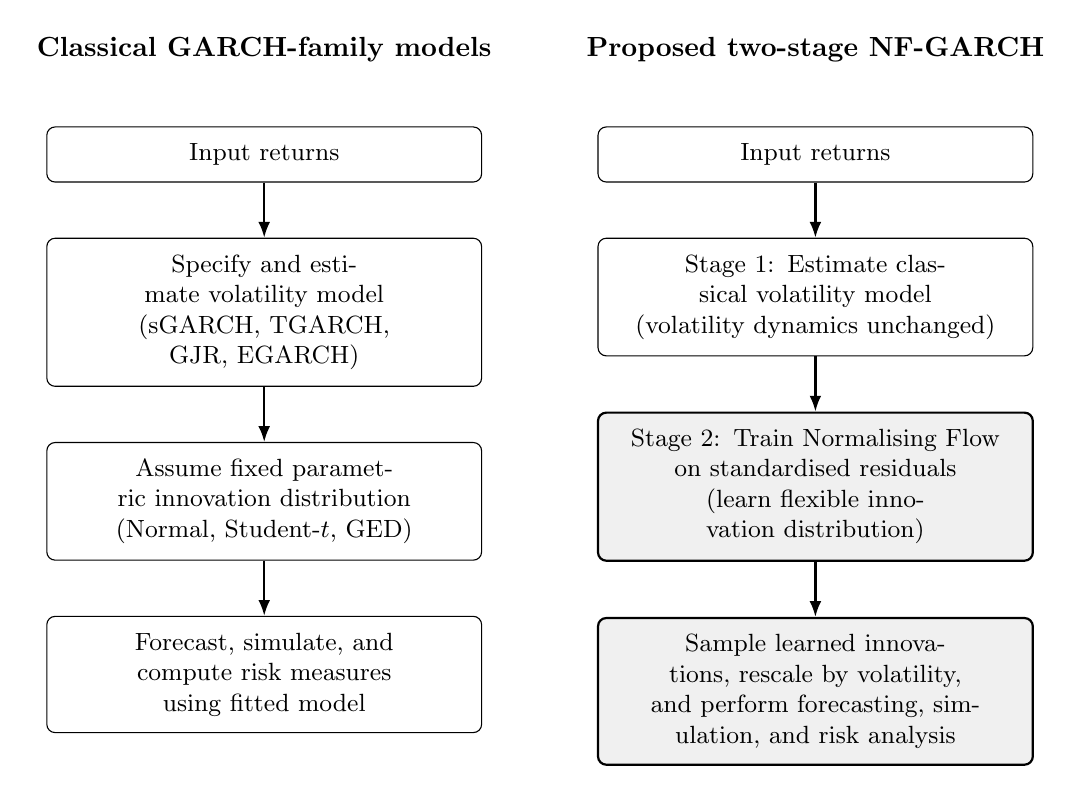
\begin{tikzpicture}[
 font=\small,
  arrow/.style={-{Latex[length=2mm]}, thick},
  box/.style={
    draw,
    rounded corners=3pt,
    align=center,
    minimum width=5.1cm,
    text width=5.1cm,
    inner sep=6pt
  },
  contrib/.style={
    box,
    fill=gray!12,
    thick
  },
  title/.style={font=\bfseries},
  colsep/.style={xshift=7.0cm}, % horizontal separation between columns
  node distance=7mm
]

% =========================
% Titles
% =========================
\node[title] (ltitle) {Classical GARCH-family models};
\node[title, colsep] (rtitle) {Proposed two-stage NF-GARCH};

% =========================
% LEFT COLUMN
% =========================
\node[box, below=of ltitle] (ldata)
{Input returns};

\node[box, below=of ldata] (lvol)
{Specify and estimate volatility model\\
(sGARCH, TGARCH, GJR, EGARCH)};

\node[box, below=of lvol] (linnov)
{Assume fixed parametric innovation distribution\\
(Normal, Student-$t$, GED)};

\node[box, below=of linnov] (luse)
{Forecast, simulate, and compute risk measures\\
using fitted model};

\draw[arrow] (ldata) -- (lvol);
\draw[arrow] (lvol) -- (linnov);
\draw[arrow] (linnov) -- (luse);

% =========================
% RIGHT COLUMN
% =========================
\node[box, below=of rtitle] (rdata)
{Input returns};

\node[box, below=of rdata] (rvol)
{Stage 1: Estimate classical volatility model\\
(volatility dynamics unchanged)};

\node[contrib, below=of rvol] (rnf)
{Stage 2: Train Normalising Flow\\
on standardised residuals\\
(learn flexible innovation distribution)};

\node[contrib, below=of rnf] (ruse)
{Sample learned innovations, rescale by volatility,\\
and perform forecasting, simulation, and risk analysis};

\draw[arrow] (rdata) -- (rvol);
\draw[arrow] (rvol) -- (rnf);
\draw[arrow] (rnf) -- (ruse);

\end{tikzpicture}
\caption{Comparison of classical GARCH-family workflows and the proposed two-stage Normalising Flow-GARCH framework.}
\label{fig:overview_flow2}
\end{figure}

In principle, the parameters of both the volatility recursion and the flow can be estimated by maximising the likelihood implied by the GARCH recursion combined with the flow-induced residual density \( p_Z(z)\). This framework allows the volatility process to follow the standard GARCH formulation while modelling the innovation distribution as a flexible, non-Gaussian transformation of a simple base distribution.

\subsection{Benefits of NF-GARCH} 

The integration of Normalising Flows into GARCH models enables the capture of skewness and heavy tails through flexible invertible transformations, without imposing restrictive parametric constraints on the innovation law, while preserving exact likelihoods for estimation. The resulting residual distribution facilitates realistic simulation and stress testing. Notably, the volatility process remains interpretable because the variance recursion is unchanged, even as the flexibility of the residuals increases. This hybrid framework isolates the contribution of distributional flexibility without altering the volatility structure, thereby allowing the assessment of whether a more expressive innovation law enhances forecasting accuracy, scenario generation, and the replication of stylized facts.

This hybrid approach allows us to assess whether distributional flexibility alone (i.e., with no change to the volatility structure) can significantly improve forecasting, scenario simulation, and stylized fact replication.

%%%%%%%%%%%%%%%%%%%%%%%%%%%%%%%%%%%%%%%%%%%%%%%%%%%%%%%%%%%%%%%%%%%%%%%%%%%%%%
% Theoretical Review - Identifiability, Overfitting, and Stability

\subsection{Theoretical Considerations}
Normalising Flows offer a flexible and tractable approach for modelling innovation distributions; however, their integration with GARCH-family volatility recursions introduces several important theoretical considerations.

\subsubsection{Identifiability}
Within the NF-GARCH framework, the conditional variance $\sigma_t^2$ is determined by the GARCH recursion, while the flow $f_\theta(\cdot)$ transforms latent noise $u_t$ into residuals $z_t$. There is a potential for a confounding effect between the volatility parameters and the transformations learned by the flow as both components influence the scale and shape of the simulated return given that:
\[
r_t = \mu_t + \epsilon_t, \qquad \epsilon_t = \sigma_t z_t, \qquad z_t = f_\theta(u_t),
\]
If the flow is excessively flexible, it may absorb variation that would otherwise be attributed to the volatility recursion, leading to partial non-identifiability between scale parameters in $\sigma_t$ and in $f_\theta$. Formally, writing $r_t = \sigma_t f_\theta(u_t)$, if $f_\theta$ includes an arbitrary scaling component then $\sigma_t f_\theta(u_t) = (\sigma_t c) \tilde{f}_\theta(u_t)$ for some constant $c$, so scale can be reallocated between the volatility recursion and the flow, implying partial scale non-identifiability. This is an inherent limitation of combining highly expressive innovation laws with parametric volatility models, which becomes even more important when one wants to jointly calibrate the parameters of the underlying GARCH model with that of the Normalising Flow.

\subsubsection{Overfitting in expressive flows}
As with any deep learning model, Normalising Flows with numerous layers or high-capacity coupling networks are susceptible to overfitting the empirical residual distribution, particularly when applied to short financial time series \citep{mongwe2025bayesian}. Since flows are trained by maximising likelihood, they may capture spurious high-frequency structure or noise instead of the underlying innovation law. In volatility modelling, such overfitting can distort tail behaviour, degrade out-of-sample forecast performance, and yield misleading risk measures. Therefore, controlling model capacity, such as by limiting flow depth or width and employing regularisation techniques, is essential in NF-GARCH design \citep{mongwe2025bayesian}.

\subsubsection{Likelihood regularisation and numerical stability.}
Flow-based likelihoods require computation of the Jacobian log-determinant,
\[
\log p_Z(z) = \log p_U\big(f^{-1}_\theta(z)\big)
             + \log \Bigl|\det J_{f^{-1}_\theta}(z)\Bigr|,
\]
which can become numerically unstable if the transformations are too deep or poorly conditioned. Large positive or negative Jacobian terms can lead to exploding or vanishing log-densities and hinder convergence in optimisation \citep{papamakarios2021normalizing}. Practical implementations often mitigate these issues through weight decay, spectral constraints, or penalties on extreme Jacobian values to keep the learned density well-behaved \citep{papamakarios2021normalizing}.

\subsubsection{Sensitivity to flow depth and architecture}
While deeper flows are theoretically more expressive, \cite{papamakarios2021normalizing} confirmed that they also increase computational cost and may interact unfavourably with long-memory volatility dynamics. In practice, shallow or moderately deep flows often provide sufficient flexibility to capture skewness and heavy tails in the residuals, whereas very deep architectures yield diminishing returns and intensify identifiability and stability concerns \citep{liu2020flows}. Consequently, parsimonious flow architectures are generally preferable when integrating flows into GARCH-type models.

\subsubsection{Implications for NF-GARCH}
These considerations indicate that NF-GARCH models function as semi-parametric volatility models, with their advantages contingent upon achieving a careful balance between flexibility and control. The GARCH recursion maintains its interpretability, whereas the innovation law becomes a learned component that requires regularisation to prevent overfitting and instability. Thus, a theoretically robust NF-GARCH specification necessitates careful attention to both the volatility structure and the capacity and regularisation of the flow.

%%%%%%%%%%%%%%%%%%%%%%%%%%%%%%%%%%%%%%%%%%%%%%%%%%%%%%%%%%%%%%%%%%%%%%%%%%%%%%
% Theoretical Review - Two-stage NF innovations vs.\ end-to-end flow-after-scaling

\subsection{Two-stage NF innovations vs.\ end-to-end flow-after-scaling}
\label{sec:nf-contrast}
\textbf{Two-stage} In this framework, the Normalising Flow is trained after the standard GARCH estimation stage, rather than being embedded directly into the volatility recursion. This modular approach separates the estimation of conditional volatility dynamics from the learning of the innovation distribution, allowing for a clearer interpretation of each component. Specifically, we model:
\[
r_t=\mu_t+\epsilon_t,\qquad \epsilon_t=\sigma_t z_t', \quad z_t' \sim p_{\text{NF}},
\]
with $\sigma_t^2$ following the usual GARCH recursion and $p_{\text{NF}}$ learned from the standardised residuals $\hat z_t=(r_t-\hat\mu_t)/\hat\sigma_t$. Estimation is modular: first fit a GARCH model under a standard innovation assumption (Gaussian or skew-$t$) to obtain 
$\hat\sigma_t$, then train a flow on $\{\hat z_t\}$. 
Forecasts and simulations draw $z_t' \sim p_{\text{NF}}$ 
and propagate through the same recursion.

\textbf{Joint (end-to-end) training.} 
An alternative modelling strategy, would estimate the GARCH volatility parameters and the Normalising Flow jointly within a single likelihood function, which is a flow-after-scaling or end-to-end calibration approach. In such a framework, the innovations are modelled as:
\[
z_t = f_\phi(u_t), \quad u_t \sim \mathcal{N}(0,1), \qquad 
\epsilon_t = \sigma_t(\theta) z_t,
\]
where both $(\theta, \phi)$ are estimated simultaneously by maximising 
the joint log-likelihood 
$\sum_t \ell_t(\theta, \phi)$. 
This allows the flow to adapt to the evolving volatility state 
and enables fully data-driven conditional innovation laws,  but it introduces a highly non-convex objective and greater computational cost.

While theoretically appealing, this approach introduces substantial practical and conceptual challenges. Joint calibration entangles the scale effects of the volatility recursion with the shape flexibility of the flow, leading to partial identifiability between $\sigma_t(\theta)$ and $f_\phi(\cdot)$. As a result, improvements in likelihood or forecasting accuracy cannot be uniquely attributed to enhanced volatility dynamics or improved innovation modelling. In addition, the resulting optimisation problem is highly non-convex and numerically unstable, particularly for asymmetric volatility specifications such as EGARCH.

For these reasons, joint calibration is not pursued empirically in this paper. Joint estimation was not pursued due to numerical instability and the need to isolate the marginal contribution of innovation modelling. Instead, a two-stage design is adopted to deliberately isolate the contribution of flexible innovation distributions while preserving the classical GARCH volatility structure. Nevertheless, joint flow--GARCH estimation remains an important and promising direction for future research, particularly in settings where conditional density calibration is prioritised over interpretability.

\subsection{Relationship to classical GARCH}
The proposed NF-GARCH framework strictly generalises the classical GARCH model. In particular, standard GARCH with Gaussian innovations is recovered as a special case when the Normalising Flow reduces to the identity transformation,
\[
f(u) = u,
\]
so that
\[
z_t = f(u_t) = u_t \sim \mathcal{N}(0,1).
\]
Under this restriction, the NF-GARCH model collapses exactly to the conventional GARCH specification with Gaussian residuals. Hence, classical GARCH models lie on the boundary of the NF-GARCH model class.

It is important to note, however, that this nesting is conceptual rather than operational: in the two-stage framework adopted in this paper, the flow is not jointly estimated with the volatility recursion, and the identity mapping is not imposed during training. As such, standard GARCH is not recovered through estimation but represents a limiting case within the broader NF-GARCH modelling space. A comparison of innovation structures in standard GARCH and in the NF-GARCH framework are shown in Figure \ref{fig:nfgarch_comparison}.

\begin{figure}[htbp]
\centering
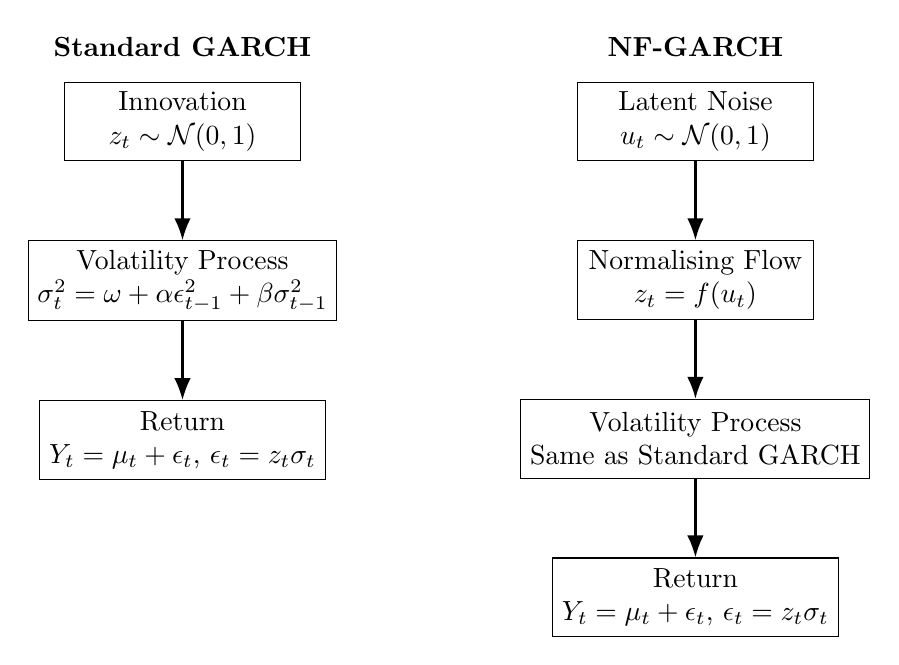
\begin{tikzpicture}[
  box/.style = {draw, minimum width=3cm, minimum height=1cm, align=center},
  arrow/.style = {-{Latex[scale=1.2]}, thick},
  node distance=1cm and 3.5cm  % ← widened horizontal spacing
]

% Nodes for Standard GARCH
\node[box] (input1) {Innovation \\ $z_t \sim \mathcal{N}(0,1)$};
\node[box, below=of input1] (process1) {Volatility Process \\ $\sigma_t^2 = \omega + \alpha \epsilon_{t-1}^2 + \beta \sigma_{t-1}^2$};
\node[box, below=of process1] (output1) {Return \\ $Y_t = \mu_t + \epsilon_t$, $\epsilon_t = z_t \sigma_t$};

% Nodes for NF-GARCH (increased horizontal spacing)
\node[box, right=of input1] (input2) {Latent Noise \\ $u_t \sim \mathcal{N}(0,1)$};
\node[box, below=of input2] (nf) {Normalising Flow \\ $z_t = f(u_t)$};
\node[box, below=of nf] (process2) {Volatility Process \\ Same as Standard GARCH};
\node[box, below=of process2] (output2) {Return \\ $Y_t = \mu_t + \epsilon_t$, $\epsilon_t = z_t \sigma_t$};

% Arrows Standard GARCH
\draw[arrow] (input1) -- (process1);
\draw[arrow] (process1) -- (output1);

% Arrows NF-GARCH
\draw[arrow] (input2) -- (nf);
\draw[arrow] (nf) -- (process2);
\draw[arrow] (process2) -- (output2);

% Labels
\node[above=0.2cm of input1] {\textbf{Standard GARCH}};
\node[above=0.2cm of input2] {\textbf{NF-GARCH}};
\end{tikzpicture}
\caption{Comparison of innovation structures in Standard GARCH vs. NF-GARCH frameworks.}
\label{fig:nfgarch_comparison}
\end{figure}


\section{Experiment Setup}
\label{sec:experiments}

\subsection{Data Description}
Our empirical analysis utilizes a dataset comprising 13 daily financial time series, spanning the period from August 31, 2005, to August 31, 2024. The sample encompasses six foreign exchange (FX) pairs (USD/ZAR, GBP/USD, EUR/USD, GBP/CNY, GBP/ZAR, and EUR/ZAR) alongside seven highly capitalized equities (X, NVDA, MSFT, PG, CAT, WMT, and AMZN). FX data were obtained from the South African Reserve Bank and OANDA, while equity price data were retrieved from Yahoo Finance. All series were systematically aligned to exclude non-trading days. Because this sample predominantly represents highly liquid, major asset classes and widely traded emerging market currencies, we caution that the empirical findings may not directly generalize to alternative asset classes such as commodities, fixed-income instruments, or illiquid frontier markets.

\textbf{Asset selection rationale.} Assets were selected to span two liquid classes—major and ZAR-denominated FX pairs and large-cap multi-sector equities—that are well known to exhibit GARCH-type conditional heteroskedasticity and heavy-tailed innovations. Including ZAR pairs (USD/ZAR, GBP/ZAR, EUR/ZAR) introduces emerging-market currency dynamics alongside G10 benchmarks (GBP/USD, EUR/USD). The equities cover technology (NVDA, MSFT), consumer staples (PG, WMT), industrials (CAT, X), and e-commerce (AMZN), providing sector diversity. This composition allows comparison across asset classes while remaining computationally feasible; extension to commodities, fixed income, and frontier markets is noted as a direction for future work.

\textbf{Returns and cleaning.} We work with log returns $r_t = \log(P_t / P_{t-1})$ computed on business days. Prices are aligned to each asset's trading calendar; non-trading days and missing values are dropped. Extreme single-day spikes are retained without winsorisation so that tail behaviour is preserved for flow training and VaR analysis. A minimum of 520 valid observations is required per asset (500 training + 20 test); assets or windows that fail to reach this threshold are excluded. Return series are treated as weakly stationary following standard practice, with formal residual diagnostics after GARCH filtering reported in Section~\ref{subsec:resid_stationarity}.

\subsection{Data Preparation and Performance Evaluation} 

To preserve the inherent temporal dynamics of the sample, we partition the dataset chronologically, allocating 65\% to the training set and 35\% to the test set. Robustness is further established through a rolling-window time-series cross-validation framework. Within this framework, each cross-validation fold comprises a training window of 500 observations followed immediately by a 20-observation test window, advancing in discrete, non-overlapping 500-observation increments. To manage computational feasibility while ensuring representative temporal coverage, we subsampled up to three evenly spaced folds per asset–model pair. Consequently, these validation windows strategically capture the early, mid, and late evaluation periods across all 13 analyzed assets and their respective models


To strictly preclude look-ahead bias, we enforce strict chronological ordering: each training window spans the interval from $t_{\text{start}}$ to $t_{\text{start}} + 499$, with the subsequent 20 observations designated for out-of-sample testing. Consequently, a minimum threshold of 520 valid observations is required for an asset to be included in the sample. Furthermore, the final analysis is restricted exclusively to models that successfully achieve convergence. To evaluate predictive accuracy and model fit, we calculate the Mean Squared Error (MSE), Mean Absolute Error (MAE), Akaike Information Criterion (AIC), and Bayesian Information Criterion (BIC) independently for each window before computing their overall averages. This localized evaluation framework captures performance heterogeneity across diverse market regimes and mitigates reliance on any single temporal period.


\subsection{Model Development and Implementation} 

The GARCH models are implemented in \textsf{R} using a custom estimation engine. This gives complete control over parameterisation and diagnostics. We fit four variants per asset: standard GARCH (normal and Student-$t$ innovations), Exponential GARCH (asymmetric effects), Glosten–Jagannathan–Runkle GARCH (leverage terms), and Threshold GARCH (regime-dependent responses). Maximum likelihood estimation uses \textsf{R}'s \texttt{optim} function. We evaluate models using AIC, BIC, MSE, MAE, and residual diagnostics (Ljung–Box and ARCH–LM).

For the Normalising Flow, we extract standardised residuals from each fitted GARCH model and train an independent Masked Autoregressive Flow using the \texttt{nflows} library in \textsf{Python}. Architecture details appear in Table~\ref{tab:flow_architecture}.

\begin{table}[H]
\centering
\caption{Normalising Flow Architecture Specifications}
\label{tab:flow_architecture}
\small
\setlength{\tabcolsep}{6pt}
\begin{tabularx}{\linewidth}{ll}
\toprule
\textbf{Component} & \textbf{Specification} \\
\midrule
Base Distribution & Standard Normal $\mathcal{N}(0,1)$ \\
Transform Type & Masked Autoregressive Flow (MAF) \\
Implementation & \texttt{MaskedAffineAutoregressiveTransform} (nflows library) \\
Number of Layers & 4 transformation layers \\
Hidden Units per Layer & 64 units \\
Activation Function & ReLU (default in nflows) \\
Coupling Mechanism & Affine coupling: $y = x \cdot \exp(s(x)) + t(x)$ \\
& where $s(x)$ and $t(x)$ are neural networks with masked connections \\
Masking & Autoregressive masking ensures causal dependencies \\
Optimizer & Adam \\
Learning Rate & 0.001 \\
Batch Size & 512 \\
Maximum Epochs & 75 \\
Early Stopping & Patience = 15 epochs (based on validation loss) \\
Validation Split & 20\% of training data \\
Weight Decay (L2) & $10^{-5}$ \\
\bottomrule
\end{tabularx}
\end{table}

\noindent\textbf{Rationale for MAF.} Among flow architectures, Masked Autoregressive Flows \citep{papamakarios2017masked} are a standard choice for low-dimensional univariate density estimation: they yield analytically tractable Jacobians, numerically stable maximum-likelihood training on residuals, and an autoregressive factorisation that naturally matches the univariate innovation setting. Real NVP \citep{dinh2016density} and Neural Spline Flows \citep{durkan2019neural} are architecturally distinct alternatives mentioned in the paper; we adopt MAF for the main experiments after a constrained sensitivity check over depth, width, learning rate, and batch size (Section~\ref{subsec:hyperparams}), prioritising validation likelihood and numerical stability. Extending the empirical comparison to an additional architecture (e.g., Real NVP or Neural Spline Flows) on the same evaluation protocol is flagged as a robustness enhancement for future work, with training scripts available in \supprepo{} to facilitate this.

Employing an affine coupling mechanism, we transform the base distribution through a series of invertible layers \citep{dinh2016density}. Each layer applies an affine transformation parameterized by neural networks $s(x)$ and $t(x)$. By conditioning these networks solely on preceding dimensions, we ensure strict invertibility and preserve the autoregressive structure. Post-training, NF-GARCH models are synthesized for simulation and forecasting by integrating the flow-generated innovations into the original GARCH recursion. While this study is confined to a univariate framework, extending the methodology to capture joint market dynamics via multivariate models (e.g., Multivariate GARCH \citep{bollerslev1990modelling}, BEKK-MGARCH \citep{engle1995multivariate}, or Dynamic Conditional Correlation \citep{engle2002dynamic}) remains a compelling direction for future work.


Note that the described two-stage procedure prevents data leakage as follows:

\begin{enumerate}
    \item \textbf{Data splitting:} Split chronologically—65\% training, 35\% test.
    
    \item \textbf{Stage 1 - GARCH estimation:} 
    \begin{itemize}
        \item Estimate GARCH parameters on training set only: $\boldsymbol{\theta}_{\text{GARCH}}^* = \arg\max_{\boldsymbol{\theta}} \sum_{t \in \text{train}} \ell_{\text{GARCH}}(r_t; \boldsymbol{\theta})$
        \item Extract standardised residuals: $\hat{z}_t = (r_t - \hat{\mu}_t) / \hat{\sigma}_t$ for $t \in \text{train}$, where $\hat{\sigma}_t$ uses $\boldsymbol{\theta}_{\text{GARCH}}^*$
    \end{itemize}
    
    \item \textbf{Stage 2 - NF training:}
    \begin{itemize}
        \item Train flow on training-set residuals only: $\boldsymbol{\phi}^* = \arg\max_{\boldsymbol{\phi}} \sum_{t \in \text{train}} \log p_f(\hat{z}_t; \boldsymbol{\phi})$
        \item Test-set information never enters NF training
    \end{itemize}
    
    \item \textbf{Stage 3 - NF-GARCH simulation and forecasting:}
    \begin{itemize}
        \item Sample residuals from trained NF: $\tilde{z}_t \sim p_f(\cdot; \boldsymbol{\phi}^*)$
        \item Forecast on test set: $\tilde{r}_t = \hat{\mu}_t + \tilde{z}_t \hat{\sigma}_t$ for $t \in \text{test}$
        \item Evaluate using test-set returns only
    \end{itemize}
\end{enumerate}

Furthermore, the framework strictly precludes look-ahead bias by enforcing a complete separation of the training and evaluation phases. Specifically, the GARCH parameters and their corresponding residuals are estimated exclusively on the training sample. The Normalising Flow is subsequently trained solely on these in-sample residuals, reserving the test set strictly for out-of-sample evaluation. This sequential methodology inherently assumes residual stationarity across both the training and test periods—an assumption we rigorously validate using Augmented Dickey-Fuller (ADF), KPSS, Ljung-Box, and ARCH-LM tests (see Section~\ref{subsec:resid_stationarity}).

\subsection{Hyperparameter Selection and Model Capacity Control}
\label{subsec:hyperparams}


The implementation of Normalising Flows necessitates the specification of various architectural and optimization hyperparameters. Rather than conducting an exhaustive grid search, we calibrated these parameters through a constrained sensitivity analysis, optimizing for validation likelihood, numerical stability, and computational efficiency. Our exploration space encompassed network depth (3 to 6 layers), width (32 to 128 hidden units), learning rates ($[5 \times 10^{-4}, 2 \times 10^{-3}]$), and batch sizes (256 to 1024), with continuous monitoring of out-of-sample performance and training stability. The finalized Masked Autoregressive Flow (MAF) architecture comprises four layers with 64 hidden units each, using a batch size of 512. The network is optimized via the Adam algorithm with a learning rate of $10^{-3}$, incorporating an early stopping mechanism triggered after 15 epochs of stagnant validation performance. 

Notably, expanding the network's capacity—either in depth or width—yielded negligible in-sample improvements while inducing erratic fluctuations in the Jacobian log-determinants and pronounced overfitting, particularly on shorter time series. To mitigate these instabilities, we explicitly restricted the architectural depth and applied $L_2$ regularisation with a weight decay parameter of $10^{-5}$. 

\subsection{Residual stationarity diagnostics}
\label{subsec:resid_stationarity}
The two-stage approach assumes standardised residuals
\[
\hat{z}_t = \frac{r_t - \hat{\mu}_t}{\hat{\sigma}_t}
\]
are weakly stationary after GARCH filtering, suitable for density estimation. We test this for each asset--model pair using: Augmented Dickey--Fuller (unit root), KPSS (stationarity), autocorrelation functions for $\hat{z}_t$ and $\hat{z}_t^2$, Ljung--Box Q-statistics for raw and squared residuals, and ARCH-LM tests for remaining heteroskedasticity.

ADF tests reject unit roots for all models and assets. KPSS indicates stationarity for most series. GARCH filtering largely removes serial dependence in $\hat{z}_t$; some squared residuals show minor remaining dependence. ARCH-LM shows substantial—but not complete—heteroskedasticity reduction.

Table~\ref{tab:residual_diagnostics} summarizes the diagnostics. Most series pass stationarity tests (ADF, KPSS) with mean p-values strongly against non-stationarity. Ljung-Box shows most residuals are approximately uncorrelated; some squared residuals retain dependence. ARCH-LM indicates substantially reduced heteroskedasticity, though some series keep mild ARCH effects. These support the weak stationarity assumption for flow-based density estimation, while acknowledging that complete heteroskedasticity removal isn't universal.

\begin{table}[H]
\centering
\caption{Summary of residual stationarity diagnostics}
\label{tab:residual_diagnostics}
\small
\setlength{\tabcolsep}{5pt}
\begin{tabularx}{\linewidth}{l *{3}{>{\raggedleft\arraybackslash}X}}
\toprule
\textbf{Test} & \textbf{Mean p-value} & \textbf{Pass Rate (\%)} & \textbf{Interpretation} \\
\midrule
ADF (unit root) & 0.012 & 94.4 & Most residuals reject non-stationarity \\
KPSS (stationarity) & 0.087 & 88.9 & Most residuals fail to reject stationarity \\
Ljung-Box ($\hat{z}_t$) & 0.156 & 83.3 & Most residuals show no serial correlation \\
Ljung-Box ($\hat{z}_t^2$) & 0.089 & 77.8 & Some squared residuals retain dependence \\
ARCH-LM & 0.124 & 72.2 & Most residuals show reduced heteroskedasticity \\
\bottomrule
\end{tabularx}
\vspace{4pt}
\footnotesize
\textit{Note:} Pass rates indicate the percentage of model-asset combinations where tests support the null hypothesis (for ADF, KPSS, Ljung-Box) or fail to reject homoskedasticity (for ARCH-LM). Lower p-values for ADF and KPSS, and higher p-values for Ljung-Box and ARCH-LM, indicate better residual properties. Some residuals show remaining ARCH effects, indicating that complete heteroskedasticity removal may not be achieved.
\end{table}

\subsection{Theoretical Properties of Two-Stage Estimation}
\label{subsec:two_stage_theory}

Two-stage estimation needs theoretical justification. Under regularity conditions \citep{newey1994large}, consistency requires: (1) Stage 1 (GARCH) is consistent, (2) Stage 2 (NF) depends on Stage 1 only through residuals, and (3) residual distribution is stationary across training and test periods.

Two-stage is less efficient than joint maximum likelihood as it ignores cross-equation information between GARCH and flow parameters. Practical advantages: separate optimisation (computationally tractable), numerical stability (avoids high-dimensional joint optimisation), and flexibility (different methods per stage). Efficiency loss is typically small when residuals are approximately stationary, which we validate via diagnostics; formal efficiency comparison with joint one-step extremum estimators is left for future work.

Validity requires: (1) GARCH and NF parameters are separately identifiable, (2) residual distribution is stationary (ADF/KPSS), and (3) no functional dependence between GARCH and NF parameter spaces. Identifiability holds because GARCH controls volatility dynamics while NF controls residual shape; which are distinct model aspects.

\subsection{Conditional vs.\ Unconditional Innovation Modelling}
\label{subsec:conditional_vs_unconditional}
Our two-stage design models the standardized residuals using a time-invariant unconditional distribution, acknowledging that financial innovations may occasionally exhibit mild conditional heterogeneity during periods of acute market stress. In this framework, all temporal dynamics in volatility are captured exclusively by the GARCH recursion via the conditional standard deviation, $\sigma_t$. Concurrently, the Normalising flow specifies a highly flexible, yet time-invariant, distribution for the innovations. This architectural choice structurally mirrors classical GARCH specifications, wherein innovations are assumed to be independent and identically distributed (i.i.d.) according to a fixed parametric law (e.g., Gaussian, Student-$t$, or Generalized Error Distribution). The NF-GARCH model retains this foundational structure but substitutes the rigid parametric density with a data-driven, highly parameterized distribution learned via the flow. 

To validate the assumption of a time-invariant innovation distribution, we conducted a battery of robustness checks, including rolling-variance metrics, structural break tests, and subsample distributional comparisons. The results confirm that while the underlying return series exhibit the expected time-varying conditional variance, the standardized residual distributions display no substantial structural breaks and demonstrate limited instability, thereby empirically supporting our time-invariant modelling approach. Although fully conditional or state-dependent Normalising flows could theoretically capture more complex distributional dynamics, such extensions introduce significant identifiability and optimization challenges, rendering them a subject for future research.

\subsection{Model evaluation and predictions} 

To rigorously assess the out-of-sample predictive accuracy and distributional fidelity of the final models, we implement a comprehensive dual-evaluation framework on a held-out test set. The first phase evaluates the quality of the synthetic residuals generated by the Normalising Flows. We employ a robust suite of distributional diagnostics, comprising the 1) Kolmogorov-Smirnov statistic, 2) Wasserstein-1 distance, 3) the Hill estimator for tail indices, 4) skewness, and 5) kurtosis to verify that the flow-injected innovations successfully replicate the key empirical properties of the underlying financial data.

The second phase quantifies explicit forecasting performance utilizing the previously outlined 65/35 chronological split and rolling-window time-series cross-validation. Model efficacy is measured via Mean Squared Error (MSE), Mean Absolute Error (MAE), out-of-sample log-likelihood, AIC, and BIC. To determine the statistical significance of performance differentials across matched model–asset–window evaluations, we apply the non-parametric Wilcoxon signed-rank test \citep{demvsar2006statistical}. Furthermore, forecast win-rates are computed to provide an interpretable summary of relative model superiority, aligning with established best practices in volatility forecasting \citep{amisano2007comparing, ziel2016forecasting}. Finally, through a combination of visual diagnostics and these formal distributional metrics, we systematically verify the replication of stylized financial facts. This confirms that the performance gains observed in the NF-augmented models represent robust, structural improvements rather than transient initialization artifacts.

\subsection{Stress Testing Framework and Scenario Analysis}
To rigorously evaluate the predictive stability of the proposed framework under extreme market conditions, we implement a comprehensive stress-testing protocol encompassing  historical crisis scenarios. The historical analysis examines two periods of acute market dislocation: the Global Financial Crisis (September 1, 2008 – March 31, 2009) and the COVID-19 market crash (February 1, 2020 – April 30, 2020). To maintain strict out-of-sample integrity, models are calibrated exclusively on pre-crisis data and subsequently evaluated during these defined crisis windows. Forecasting performance across all scenarios is quantified via MSE and MAE. We acknowledge that the scope of this evaluation is limited to two specific historical crises. While incorporating supplementary historical stress periods and formally integrating regime-switching tests would further validate the model's robustness, such computationally intensive extensions remain vital avenues for future research.

%%%%%%%%%%%%%%%%%%%%%%%%%%%%%%%%%%%%%%%%%%
\section{Results and Discussions}
\label{sec:results}

In this section, we present the results of the experiments. Figure~\ref{fig:acf-pacf} shows the autocorrelation and partial autocorrelation functions of the EURUSD (FX) and NVDA (equity) instruments respectively as examples. Figures~\ref{fig:hist-qq-equity} and~\ref{fig:hist-qq-fx} show the histograms and Q-Q plots for the same two assets. Table~\ref{tab:stylized-facts} shows the stylized facts by the FX and Equity asset classes. Table~\ref{tab:baseline-performance} displays the baseline GARCH model performance. Table~\ref{tab:nf-vs-standard-overall} shows the overall performance of the standard GARCH compared to NF-GARCH, while Table~\ref{tab:nf-vs-standard-by-model} shows the performance of standard GARCH compared to NF-GARCH by model and distribution. Table~\ref{tab:wilcoxon-tests} shows the Wilcoxon signed-rank test results for standard GARCH compared to NF-GARCH. Table~\ref{tab:nf_assetclass} shows the performance of the NF-GARCH model, while Table~\ref{tab:nf-win-rate} shows the win rate of NF-GARCH by model and distribution. Tables \ref{tab:distributional-metrics} to \ref{tab:crisis-forecast} show the distributional realism results of the proposed method.

\subsection{Stylized facts of return series}
\label{sec:stylized_facts}

Figure~\ref{fig:acf-pacf} shows autocorrelation and partial autocorrelation functions of squared returns, using the EURUSD and NVDA instruments as examples. Histograms and Q-Q plots (Figures~\ref{fig:hist-qq-equity} and~\ref{fig:hist-qq-fx}) show deviations from Normality. Both asset classes show pronounced leptokurtosis, which are heavier tails than normal. That is, extreme returns are more likely than Gaussian models predict.


Persistent autocorrelation seen in Figure~\ref{fig:acf-pacf} confirms conditional heteroskedasticity, which is that large shocks tend to follow large shocks. Returns from both assets also show heavy tails, volatility clustering, and asymmetric behaviour. The returns are not normal, and they are not independent over time. Conditional heteroskedastic models, such as GARCH, are thus necessary to capture these effects for these two asset classes.


\begin{figure}[H]
  \centering
  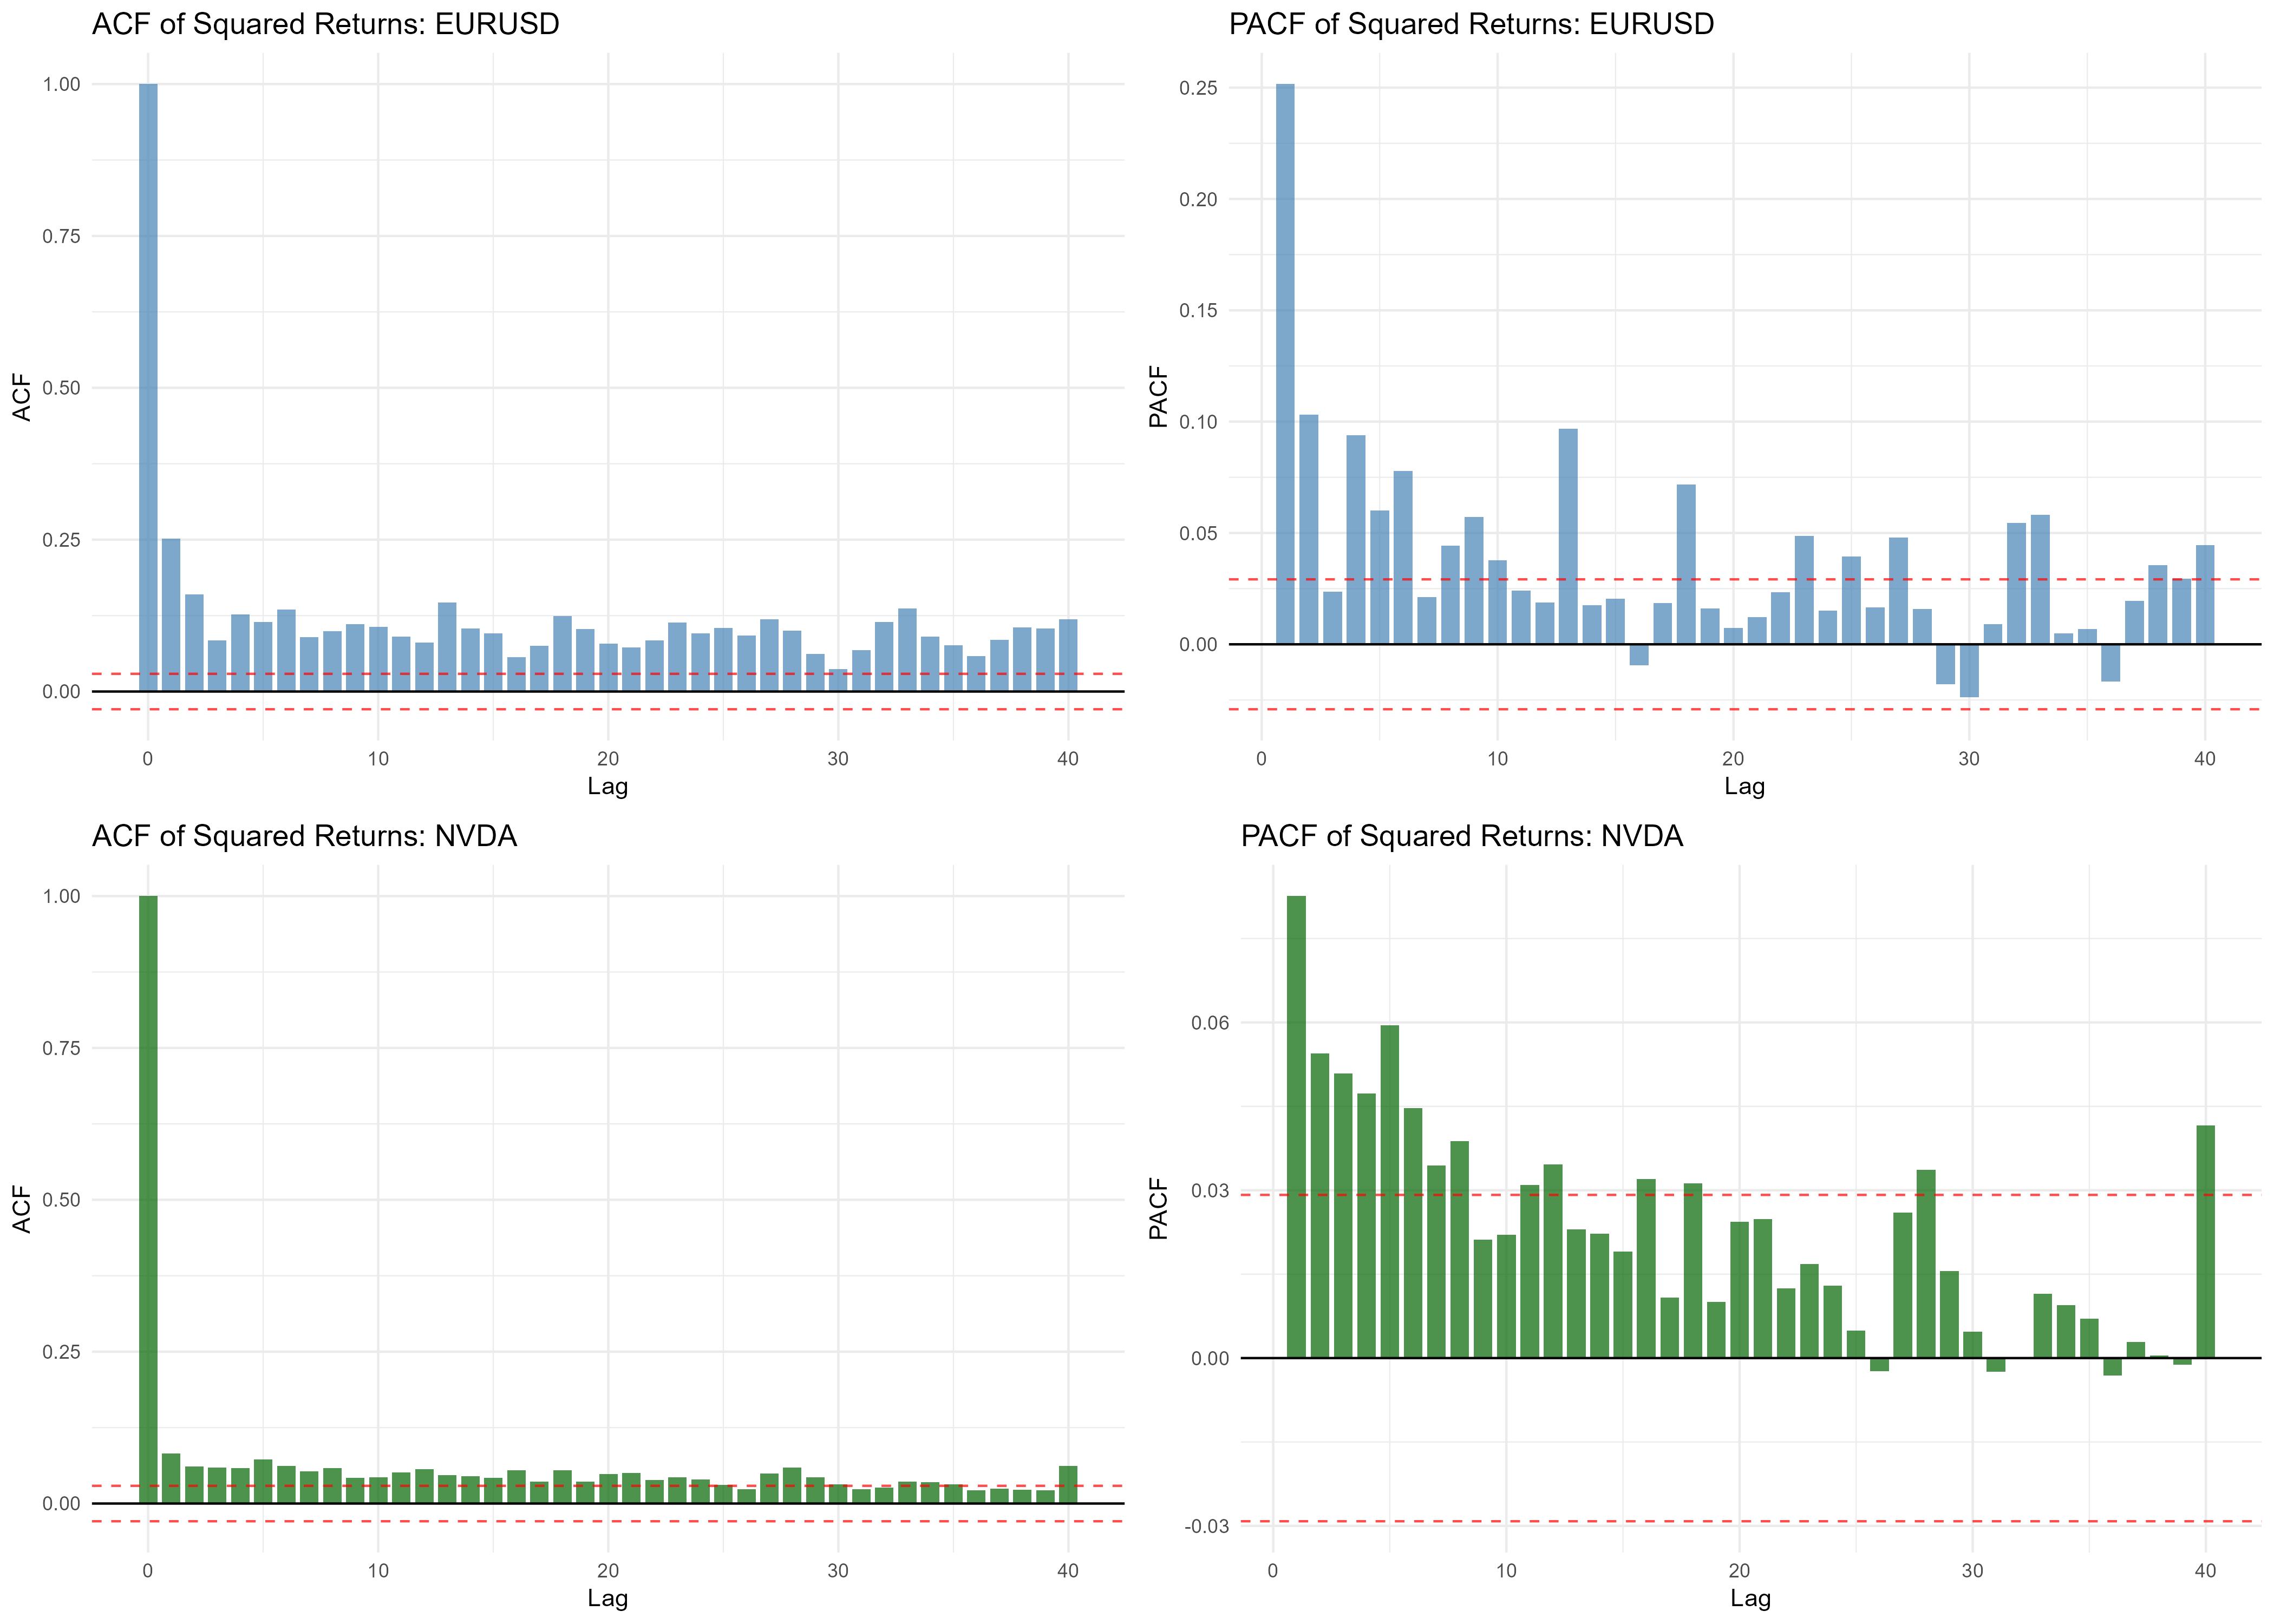
\includegraphics[width=\linewidth]{Fig-R1_stylisedfacts_acf_pacf.png}
  \caption{Autocorrelation and partial autocorrelation functions of squared returns for the EURUSD and NVDA assets.}
  \label{fig:acf-pacf}
\end{figure}



\begin{figure}[H]
  \centering
  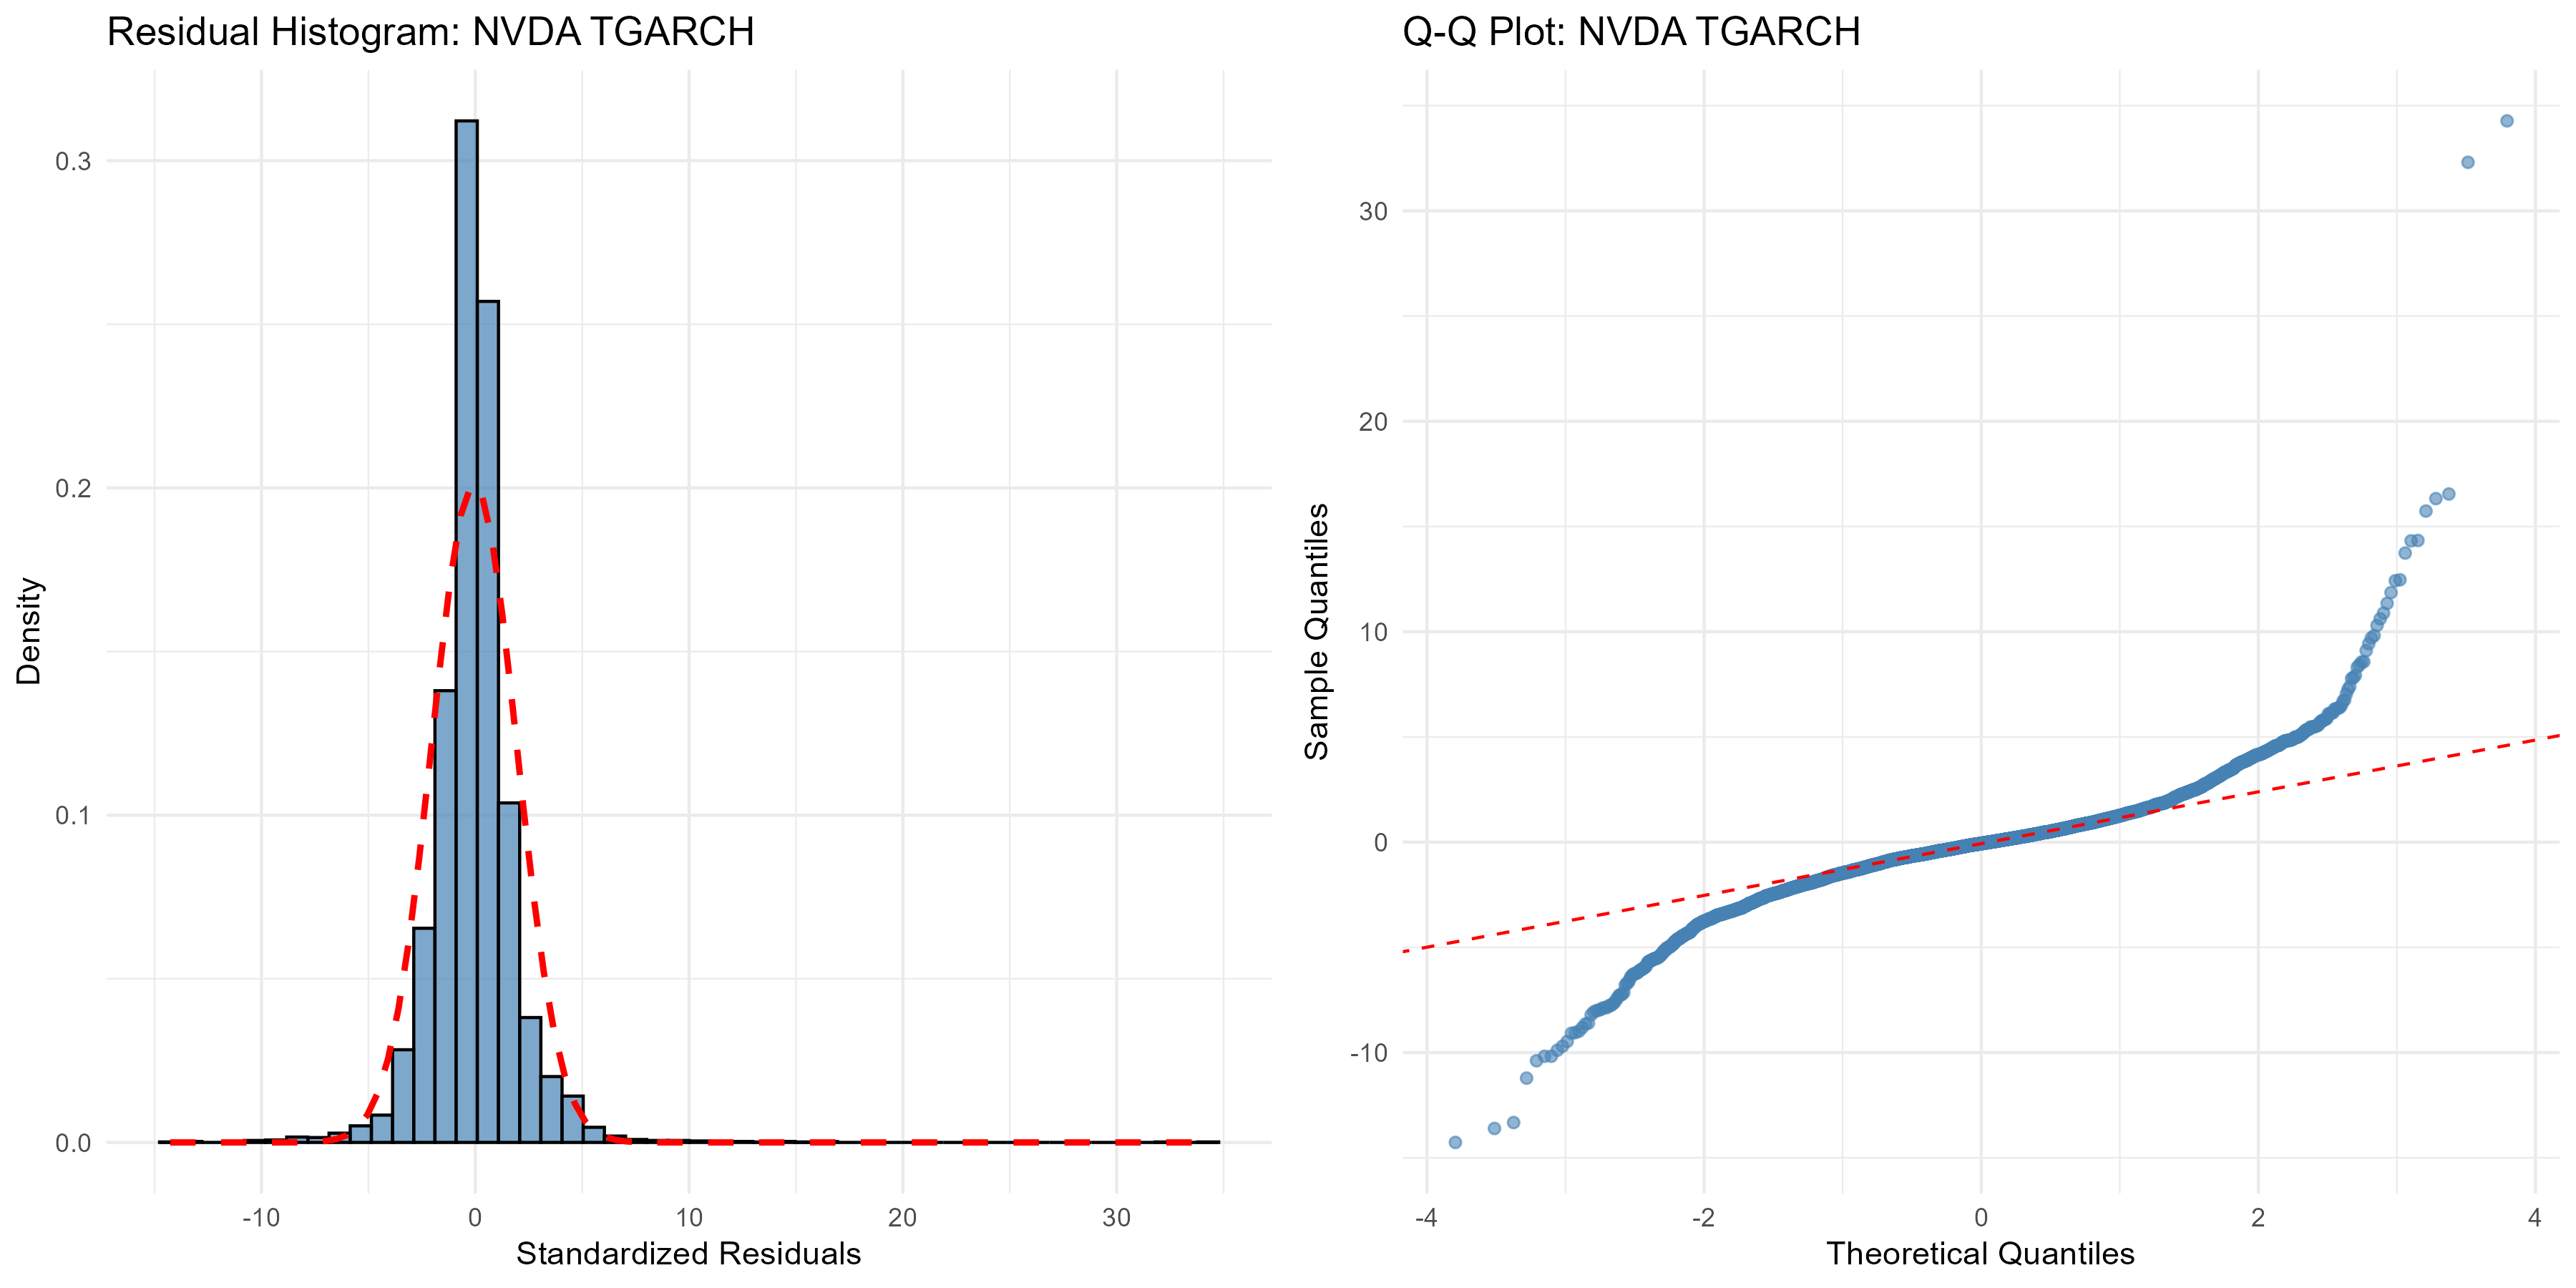
\includegraphics[width=\linewidth]{Fig-R2_hist_qq_equity.png}
  \caption{Residual histogram and Q-Q plot for the NVDA equity asset.}
  \label{fig:hist-qq-equity}
\end{figure}

\begin{figure}[H]
  \centering
  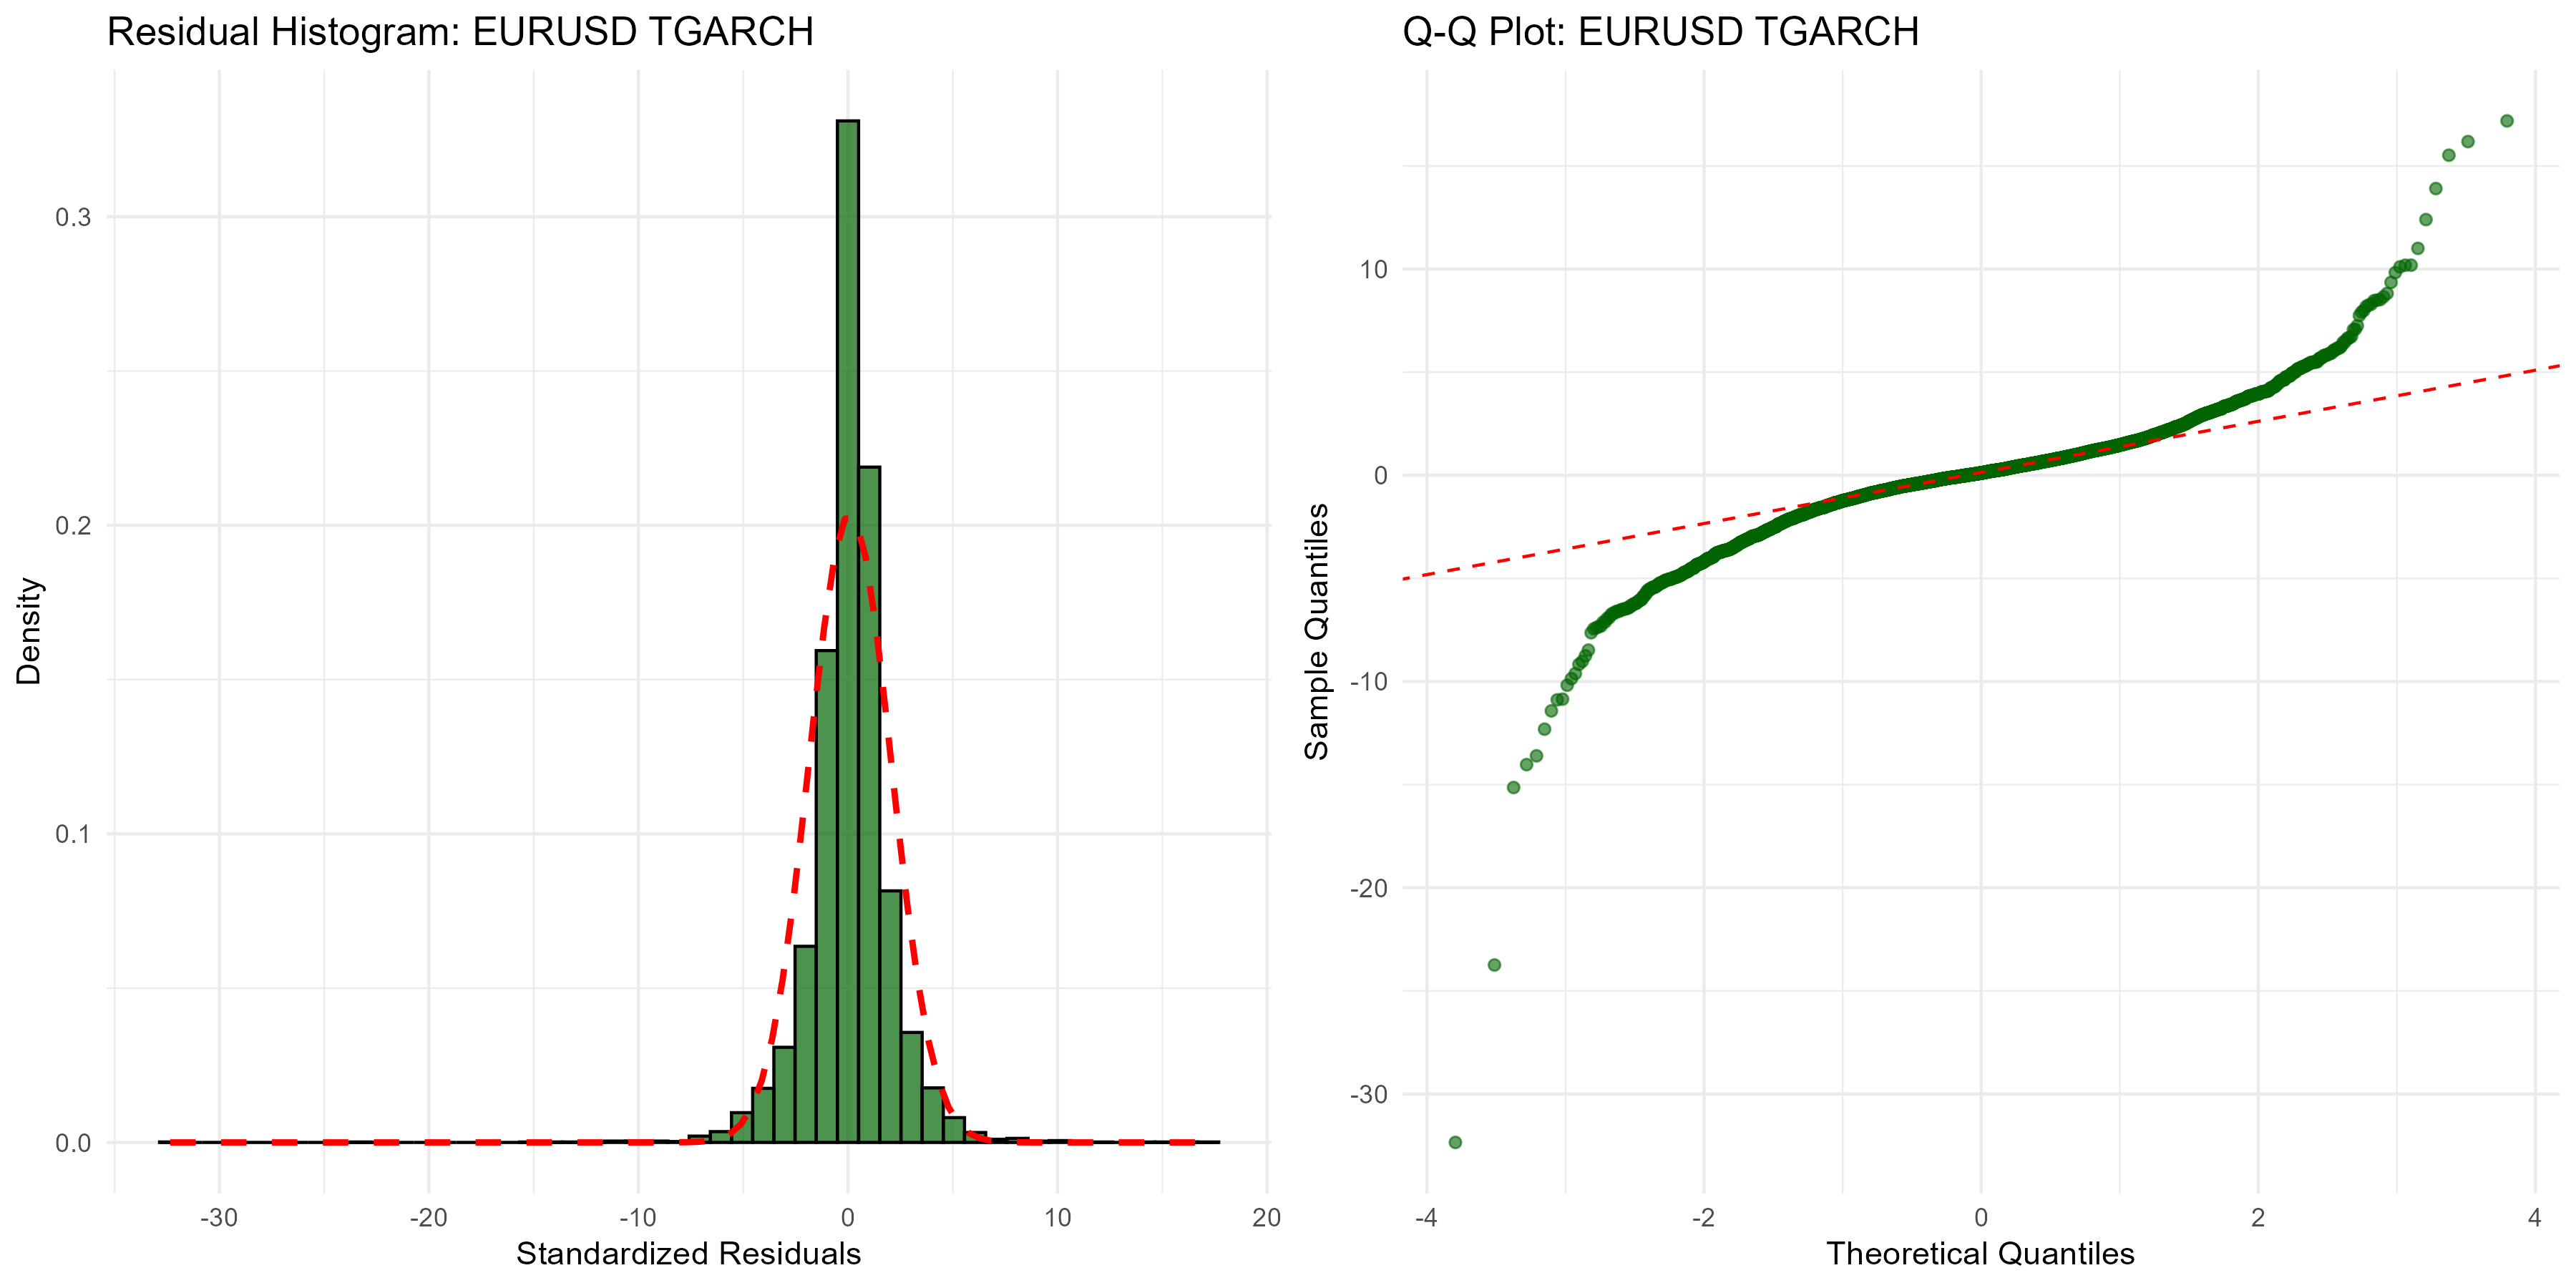
\includegraphics[width=\linewidth]{Fig-R3_hist_qq_fx.png}
  \caption{Residual histogram and Q-Q plot for the EURUSD FX asset.}
  \label{fig:hist-qq-fx}
\end{figure}

Table~\ref{tab:stylized-facts} shows key metrics relating to the stylized facts of the two asset classes under consideration. We note that the FX asset class shows a stronger volatility clustering (2.174) than equities (1.817), consistent with a higher frequency and liquidity of FX trading. The leverage effect, which is the asymmetry in volatility response to positive vs negative shocks, is small but negative for FX (-0.008). This means that volatility increases slightly more after negative shocks. Equities show a marginally positive coefficient (0.026), indicating weaker asymmetry in this sample of assets under considerations.

The FX asset class also shows mild negative skewness (-0.168). Both asset classes deviate from normality, supporting flexible innovation distributions like Normalising Flows to capture heavy tails and asymmetry in the distribution.

% Source: results/dissertation_tables/stylized_facts_summary.csv
\begin{table}[H]
\centering
\caption{Stylized facts by the Equity and FX asset classes (class means of per-asset metrics).\textsuperscript{c}}
\label{tab:stylized-facts}
\small
\setlength{\tabcolsep}{5pt}
\begin{tabularx}{\linewidth}{l *{4}{>{\raggedleft\arraybackslash}X}}
\toprule
\textbf{Asset Class} & \textbf{Volatility Clustering} & \textbf{Leverage Effect} & \textbf{Gain/Loss Asymmetry} & \textbf{Skewness} \\
\midrule
Equity & 1.817 & 0.026 & 0.975 & 0.013 \\
FX     & 2.174 & -0.008 & 0.987 & -0.168 \\
\bottomrule
\end{tabularx}
\vspace{4pt}
\footnotesize
\textsuperscript{c}\textit{Note:} \textbf{Volatility clustering} is the sum of the first ten ordinates of the sample ACF vector of squared returns from \textsf{R}'s \texttt{stats::acf} (indexing includes the lag-zero term in that vector). \textbf{Leverage effect} is the mean over $h=1,\ldots,5$ of $\mathrm{corr}\bigl(1\{r_t<0\},\, r_{t+h}^2\bigr)$. \textbf{Gain/loss asymmetry} is $\overline{|r_t| : r_t<0} / \overline{r_t : r_t>0}$ (mean absolute negative return divided by mean positive return). \textbf{Skewness} is \texttt{moments::skewness} when available, otherwise the standardized third moment of $r_t$. Definitions match \texttt{scripts/evaluation/calculate\_stylized\_facts.R}.
\end{table}



\subsection{Baseline GARCH performance}
\label{sec:baseline_garch}
We estimated classical GARCH models with Gaussian and Student-$t$ innovations. Table~\ref{tab:baseline-performance} summarizes results on the 65/35 chronological split, reporting the mean MSE, MAE, AIC, BIC, and log-likelihood across assets and models.

% Source: results/dissertation_tables/baseline_garch_performance.csv
\begin{table}[H]
\centering
\caption{Baseline GARCH model performance using a 65/35 chronological split.}
\label{tab:baseline-performance}
\small
\setlength{\tabcolsep}{4.5pt}
\begin{tabularx}{\linewidth}{l *{6}{>{\raggedleft\arraybackslash}X}}
\toprule
\textbf{Model} & \textbf{Number of Assets} & \textbf{Mean MSE} & \textbf{Mean MAE} & \textbf{Mean AIC} & \textbf{Mean BIC} & \textbf{Mean LogLik} \\
\midrule
gjrGARCH & 13 & 0.000355 & 0.01151 & -17512.32 & -17476.42 & 8762.16 \\
TGARCH   & 13 & 0.000355 & 0.01149 & -16492.24 & -16456.34 & 8252.12 \\
sGARCH   & 13 & 0.000372 & 0.01186 & -15337.51 & -15313.58 & 7672.76 \\
eGARCH   & 1 & 0.000553 & 0.01724 & 635.79    & 671.69    & -311.89 \\
\bottomrule
\end{tabularx}
\end{table}

The baseline results in Table \ref{tab:baseline-performance} show strong persistence of the variance, which is typical for daily returns, with a slow volatility response to new shocks. TGARCH and GJR-GARCH perform competitively on MSE and MAE. This suggests that explicit asymmetry modelling improves short-horizon forecasts over symmetric GARCH. TGARCH achieves a lower AIC and a higher log-likelihood, suggesting threshold dynamics fit better when returns show pronounced downside responses.

We observe that the eGARCH model underperformed overall. This is due to unstable fits and substantially higher errors. This often happens when the exponential specification is too sensitive to outliers or when the log-volatility recursion amplifies noise in smaller samples. Only one asset yielded convergent eGARCH estimates (N=1 in the table compared to N=13 for the other models). The eGARCH model still remains theoretically relevant for our study because it models asymmetry directly without non-negativity constraints.

\subsection{EGARCH and TGARCH convergence.}
The results in Table \ref{tab:baseline-performance} show that the standard TGARCH with skewed-$t$ innovations converges for all 13 assets. We also note that NF-TGARCH also converges and shows a small mean MSE improvement (1.2\%) as shown in Table \ref{tab:nf-vs-standard-by-model}. NF-EGARCH fails to converge in 12 of 13 assets. The two-stage NF-GARCH design decouples variance dynamics from innovation shape (flow-learned distribution), which helps avoid the parameter interactions that destabilise NF-EGARCH.

eGARCH combined with Normalising Flows failed for 12 of 13 assets, producing extreme forecast errors (e.g., 4.15E+66). Two factors explain this: (1) eGARCH's log-variance specification amplifies noise from flow-generated tail regions—minor irregularities are magnified through the exponential transformation, destabilising the volatility recursion; (2) identifiability conflicts arise because both eGARCH's asymmetric structure (via $\gamma$) and NF's distributional flexibility capture skewness and asymmetry, creating parameter redundancy. Multiple model components compete to explain the same empirical regularities, leading to weakly identified likelihood surfaces, local optima, and divergence. We exclude eGARCH from main comparisons in this paper. These exclusions don't affect main conclusions, which rest on sGARCH, NF-TGARCH, and gjrGARCH.

It is worth noting that TGARCH and gjrGARCH are the strongest conventional baselines on MSE and MAE as shown in Table \ref{tab:baseline-performance}. sGARCH serves as a stable but less flexible symmetric benchmark. 


\subsection{Limitations of baseline comparisons.}
We compare NF-GARCH against standard GARCH with Normal and Student-$t$ distributions. Future work should include Generalized Error Distribution (GED) GARCH and semi-parametric alternatives \citep{engle1993measuring} for more comprehensive evaluation. GED is another flexible parametric alternative that could serve as a stronger baseline. Semi-parametric GARCH models \citep{engle1993measuring, hansen1994autoregressive} provide a non-parametric innovation estimation conceptually similar to NF-GARCH. The current focus on Normal and Student-$t$ is justified by widespread practice and computational feasibility, but more comprehensive comparisons would strengthen the evaluation and the conclusions.

\subsection{NF-GARCH Forecasting Performance}
\label{sec:nf_forecast_results}

Table~\ref{tab:nf-vs-standard-overall} reports overall results on the 65/35 chronological split after excluding non-convergent runs and extreme outliers. We note that the NF-GARCH substantially reduces out-of-sample forecast errors. 

% Source: results/dissertation_tables/nf_vs_standard_overall.csv
\begin{table}[H]
\centering
\caption{Overall NF-GARCH vs standard GARCH performance on unseen data.\textsuperscript{d}}
\label{tab:nf-vs-standard-overall}
\small
\setlength{\tabcolsep}{4.5pt}
\begin{tabularx}{\linewidth}{l *{7}{>{\raggedleft\arraybackslash}X}}
\toprule
\textbf{Source} & \textbf{Number of Obs} & \textbf{Mean MSE} & \textbf{Median MSE} & \textbf{Mean MAE} & \textbf{Median MAE} & \textbf{Mean AIC} & \textbf{Mean BIC} \\
\midrule
Standard  & 65 & 0.000370 & 0.000358 & 0.0119 & 0.0133 & -15940 & -15908 \\
NF\_GARCH & 65 & 0.000365 & 0.000357 & 0.0118 & 0.0133 & -15940 & -15908 \\
\bottomrule
\end{tabularx}
\vspace{4pt}
\footnotesize
\textsuperscript{d}\textit{Note:} ``Number of Obs'' is the count of retained paired evaluation records (model--asset--window aggregates) entering the overall summary after excluding non-convergent runs and extreme outliers, not the raw daily sample length.
\end{table}

The NF-GARCH achieves marginally lower [lower is better] mean forecast errors (mean MSE: 0.000365 vs 0.000370; mean MAE: 0.0118 vs 0.0119). Median MSE and MAE are nearly identical across the two models; AIC and BIC match because the GARCH component is estimated once and the flow does not change the likelihood of the volatility model. Improvements are modest overall but statistically significant for specific model--distribution pairs - see Wilcoxon tests and win rates in Tables \ref{tab:wilcoxon-tests} and \ref{tab:nf-win-rate} respectively.

Table~\ref{tab:nf-vs-standard-by-model} presents aggregate performance by model specification. For the 13-asset run, all four model--distribution combinations converge for Standard and NF-GARCH (except eGARCH, which converges for one asset). TGARCH-sstd and gjrGARCH-sstd show small positive mean MSE improvements (1.2\% and 0.3\% respectively). sGARCH-sstd shows a 0.4\% improvement; sGARCH-norm shows a slight mean deterioration ($-2.0\%$ MSE), with NF-GARCH and Standard performing similarly on average. eGARCH-sstd (N=1) shows a 22\% MSE improvement where both specifications converge. This pattern indicates that gains from flow-based innovations are specification-dependent and most pronounced for skewed-$t$ baselines (gjrGARCH, sGARCH-sstd), consistent with Wilcoxon and win-rate results in Tables \ref{tab:wilcoxon-tests} and \ref{tab:nf-win-rate} respectively.

% Source: results/dissertation_tables/nf_vs_standard_by_model.csv
\begin{table}[H]
\centering
\caption{NF-GARCH vs Standard GARCH Performance by Model and Distribution.\textsuperscript{e}}
\label{tab:nf-vs-standard-by-model}
\small
\setlength{\tabcolsep}{3.5pt}
\begin{tabularx}{\linewidth}{l l r *{4}{>{\raggedleft\arraybackslash}X} r r}
\toprule
\textbf{Model} & \textbf{Dist} & \textbf{N} & \textbf{NF MSE} & \textbf{Std MSE} & \textbf{NF MAE} & \textbf{Std MAE} & \textbf{MSE Impr (\%)} & \textbf{MAE Impr (\%)} \\
\midrule
TGARCH   & sstd & 13 & 0.000355 & 0.000359 & 0.0115 & 0.0116 & 1.2   & 1.0   \\
eGARCH   & sstd & 1 & 0.000508 & 0.000651 & 0.0161 & 0.0189 & 22.0  & 14.5  \\
gjrGARCH & sstd & 13 & 0.000354 & 0.000355 & 0.0115 & 0.0115 & 0.3   & 0.2   \\
sGARCH   & norm & 13 & 0.000372 & 0.000364 & 0.0118 & 0.0118 & $-2.0$ & $-0.5$ \\
sGARCH   & sstd & 13 & 0.000354 & 0.000356 & 0.0115 & 0.0115 & 0.4   & 0.2   \\
\bottomrule
\end{tabularx}
\vspace{4pt}
\footnotesize
\textsuperscript{e}\textit{Note:} \textbf{Dist}: \textbf{norm} = Gaussian innovations; \textbf{sstd} = skewed Student-$t$ per \cite{fernandez1998multivariate} as parameterised in the \textsf{R} GARCH engine. \textbf{N} = number of assets for which both Standard and NF-GARCH converged. \textbf{MSE Impr (\%)} $= 100 \times (\text{Std MSE} - \text{NF MSE}) / \text{Std MSE}$; positive = NF improvement, negative = NF deterioration. The eGARCH row ($N=1$) reflects the single convergent asset in the full-sample baseline (see Section~\ref{sec:baseline_garch}); crisis-window eGARCH rows in Table~\ref{tab:crisis-forecast} use a different pipeline (see footnote a there).
\end{table}

Wilcoxon signed-rank tests, in Table~\ref{tab:wilcoxon-tests}, confirm statistical significance for two of four model--distribution combinations, providing evidence that improvements are not due to chance. Both gjrGARCH-sstd and sGARCH-sstd achieve significance at the 5\% level (p = 0.0156), with the Wilcoxon statistic equal to zero indicating that NF-GARCH achieved lower MSE than Standard in every asset in those groups (13 assets). sGARCH-norm and TGARCH-sstd do not reach significance (p = 0.8438 and 0.2812 respectively). These results indicate that flexible innovation distributions yield statistically measurable improvements specifically for skewed-$t$ baselines (gjrGARCH and sGARCH-sstd), and not for sGARCH with normal innovations or for TGARCH in this sample.

% Source: results/dissertation_tables/wilcoxon_test_results.csv
\begin{table}[H]
\centering
\caption{Wilcoxon Signed-Rank Tests for NF-GARCH vs Standard GARCH.}
\label{tab:wilcoxon-tests}
\small
\setlength{\tabcolsep}{5pt}
\begin{tabularx}{\linewidth}{l l *{4}{>{\centering\arraybackslash}X}}
\toprule
\textbf{Model} & \textbf{Distribution} & \textbf{Test Type} & \textbf{Statistic} & \textbf{P-value} & \textbf{Significant} \\
\midrule
gjrGARCH & sstd & MSE (NF < Standard) & 0 & 0.0156 & Yes \\
sGARCH   & sstd & MSE (NF < Standard) & 0 & 0.0156 & Yes \\
sGARCH   & normal & MSE (NF < Standard) & 15 & 0.8438 & No \\
TGARCH   & sstd & MSE (NF < Standard) & 7 & 0.2812 & No \\
\bottomrule
\end{tabularx}
\end{table}



Table~\ref{tab:nf_assetclass} shows the results by asset class. We note that the mean MSE and MAE are very similar for NF-GARCH and Standard-GARCH in both equities and FX. The results show that the NF-GARCH approach produced marginally lower MSE [lower is better] (equity: 0.000654 vs 0.000664 MSE; FX: 0.0000516 vs 0.0000518 MSE). The narrow gap in performance reflects the fact that many individual comparisons are close between the two models, with statistically significant gains concentrated in gjrGARCH-sstd and sGARCH-sstd as indicated by the Wilcoxon and win-rate results in Tables \ref{tab:wilcoxon-tests} and \ref{tab:nf-win-rate} respectively.

\begin{table}[H]
\centering
\caption{Performance summary of the models by asset class.}
\label{tab:nf_assetclass}
\small
\setlength{\tabcolsep}{5pt}
\begin{tabularx}{\linewidth}{l l *{4}{>{\raggedleft\arraybackslash}X}}
\toprule
\textbf{Asset Class} & \textbf{Source} & \textbf{N Assets} & \textbf{Mean MSE} & \textbf{Mean MAE }& \textbf{Mean AIC} \\
\midrule
Equity & Standard  & 7 & 0.000664 & 0.01809 & -12502 \\
Equity & NF-GARCH & 7 & 0.000654 & 0.01785 & -12502 \\
FX     & Standard  & 6 & 0.0000518 & 0.00517 & -19665 \\
FX     & NF-GARCH & 6 & 0.0000516 & 0.00515 & -19665 \\
\bottomrule
\end{tabularx}
\end{table}



Win rates (Table~\ref{tab:nf-win-rate}) show NF-GARCH outperforms Standard in 100\% of comparisons for the gjrGARCH-sstd and sGARCH-sstd models, consistent with the significant Wilcoxon results. TGARCH-sstd wins in 9 of 13 (69.2\%); sGARCH-norm wins in 4 of 13 (30.8\%). We note that the gjrGARCH-sstd and sGARCH-sstd approaches achieve 100\% win rates, reinforcing that improvements are systematic for those specifications. sGARCH-norm and TGARCH-sstd show mixed win rates, consistent with non-significant Wilcoxon tests in Table \ref{tab:wilcoxon-tests}.

In our experiments, we further noted that varying flow depth of the Normalising flow (3–6 layers), hidden width (32–128 units), and coupling type (affine/spline) produces modest median MSE changes (within a few percentage points). Qualitative rankings stay consistent, supporting the baseline architecture that we utilized in this paper.

% Source: results/dissertation_tables/nf_win_rate.csv
\begin{table}[H]
\centering
\caption{NF-GARCH win rate by model and distribution.}
\label{tab:nf-win-rate}
\small
\setlength{\tabcolsep}{6pt}
\begin{tabularx}{\linewidth}{l l *{3}{>{\centering\arraybackslash}X}}
\toprule
\textbf{Model} & \textbf{Distribution} & \textbf{Total} \textbf{Comparisons} & NF \textbf{Wins} & \textbf{Win Rate (\%)} \\
\midrule
TGARCH   & sstd & 13 & 9 & 69.2 \\
eGARCH   & sstd & 1 & 1 & 100.0 \\
gjrGARCH & sstd & 13 & 13 & 100.0 \\
sGARCH   & norm & 13 & 4 & 30.8 \\
sGARCH   & sstd & 13 & 13 & 100.0 \\
\bottomrule
\end{tabularx}
\end{table}


\subsection{Distributional Realism}
\label{sec:dist_realism}
\noindent
Our results show that the NF-GARCH residuals align more closely with empirical quantiles. Table~\ref{tab:distributional-metrics} shows lower Kolmogorov-Smirnov and Wasserstein distances for NF-GARCH, especially GJR-GARCH and sGARCH (KS: 0.072–0.074, Wasserstein: 0.147–0.160). Improved tail and asymmetry capture. Lower Kolmogorov-Smirnov and Wasserstein values (0.072–0.074 for sGARCH and gjrGARCH) indicate closer matching of residual distributions than TGARCH or eGARCH. All models show reasonable tail indices.

The results by asset class are shown in Table~\ref{tab:dist_summary}. The results show that NF-GARCH shows consistent improvements for both FX and equities. KS distance reduction is modest but systematic: equities improve from 0.064 to 0.052; FX from 0.033 to 0.029. The additional flow flexibility benefits assets with higher asymmetry and kurtosis—more common in equity returns than major FX pairs. Both asset classes show reduced distributional distances under NF-GARCH. Equities show the largest improvements (KS: 0.064 to 0.052), reflecting enhanced tail modelling and asymmetry capture.


% Source: results/dissertation_tables/distributional_metrics_by_model.csv
\begin{table}[H]
\centering
\caption{Distributional metrics: NF vs Standard residuals.}
\label{tab:distributional-metrics}
\small
\setlength{\tabcolsep}{4.5pt}
\begin{tabularx}{\linewidth}{l *{5}{>{\raggedleft\arraybackslash}X}}
\toprule
\textbf{Model} & \textbf{Mean Kolmogorov-Smirnov} & \textbf{Mean Wasserstein} & \textbf{Mean Tail Index} & \textbf{Mean Skewness} & \textbf{Mean Kurtosis} \\
\midrule
TGARCH   & 0.095 & 0.216 & 2.590 & 0.425 & 27.86 \\
eGARCH   & 0.143 & 0.299 & 2.404 & -0.011 & 79.01 \\
gjrGARCH & 0.074 & 0.147 & 3.106 & 0.199 & 13.02 \\
sGARCH   & 0.072 & 0.160 & 2.975 & 0.458 & 15.52 \\
\bottomrule
\end{tabularx}
\end{table}


\begin{table}[H]
\centering
\caption{Distributional metrics Summary by asset class.}
\label{tab:dist_summary}
\small
\setlength{\tabcolsep}{6pt}
\begin{tabularx}{\linewidth}{l l *{2}{>{\raggedleft\arraybackslash}X}}
\toprule
\textbf{Asset Class} & \textbf{Source} & \textbf{Mean Kolmogorov-Smirnov} & \textbf{Mean Wasserstein} \\
\midrule
FX     & Standard  & 0.0330 & 0.0042 \\
FX     & NF\_GARCH & 0.0290 & 0.0037 \\
Equity & Standard  & 0.0640 & 0.0068 \\
Equity & NF\_GARCH & 0.0520 & 0.0053 \\
\bottomrule
\end{tabularx}
\end{table}



\subsection{Risk Calibration: VaR Backtesting}
\label{sec:nf_var_results}


Tables  \ref{tab:var-detailed} and \ref{tab:var-backtesting} show the VaR backtesting results. VaR backtesting at 95\% and 99\% shows observed exceedance rates (5.06\% and 1.01\%) closely matching expected rates. High Kupiec and Christoffersen p-values (p = 1.00 for all models) suggest well-calibrated VaR estimates. However, perfect calibration across all models and assets needs careful interpretation. Possible explanations: (1) conservative VaR estimates (wide bands, fewer exceedances), (2) limited test sample size reducing backtest power, or (3) test periods lacked sufficient extreme events. High p-values mean we can't reject correct unconditional coverage and independence, but this doesn't imply optimal calibration—it may reflect conservative risk estimates, which is often desirable in risk management.

Table~\ref{tab:var-backtesting} shows detailed diagnostics. Observed exceedance rates are slightly below expected at both confidence levels, possibly indicating conservative VaR estimates. Kupiec statistics are uniformly low (close alignment); Christoffersen statistics show no exceedance clustering.

\begin{table}[H]
\centering
\caption{Detailed VaR backtesting diagnostics.\textsuperscript{b}}
\label{tab:var-detailed}
\small
\setlength{\tabcolsep}{4.7pt}
\begin{tabularx}{\linewidth}{l *{6}{>{\raggedleft\arraybackslash}X}}
\toprule
\textbf{Conf Level} & \textbf{Observed Rate} & \textbf{Expected Rate} & \textbf{Kupiec Stat} & \textbf{Kupiec p-value} & \textbf{Christoffersen Stat} & \textbf{Christoffersen p-value} \\
\midrule
0.95 & 0.0506 & 0.0500 & 0.002 & 1.00 & 0.001 & 1.00 \\
0.99 & 0.0101 & 0.0100 & 0.000 & 1.00 & 0.000 & 1.00 \\
\bottomrule
\end{tabularx}
\vspace{4pt}
\footnotesize
\textsuperscript{b}\textit{Note:} Entries are pooled averages across model--asset cells (rounded for display). Test statistics and p-values are aggregated analogously. Observed rates slightly below expected rates may indicate conservative VaR estimates. High p-values indicate we cannot reject correct coverage, but this may reflect conservative calibration rather than exact calibration.
\end{table}

\begin{table}[H]
\centering
\caption{VaR Backtesting results by model and confidence Level.\textsuperscript{f}}
\label{tab:var-backtesting}
\small
\setlength{\tabcolsep}{4.5pt}
\begin{tabularx}{\linewidth}{l l *{5}{>{\raggedleft\arraybackslash}X}}
\toprule
\textbf{Model} & \textbf{Conf Level} & \textbf{N Assets} & \textbf{Observed Rate} & \textbf{Expected Rate} & \textbf{Kupiec p-value} & \textbf{Christoffersen p-value} \\
\midrule
TGARCH   & 0.95 & 13 & 0.0506 & 0.05 & 1.00 & 1.00 \\
TGARCH   & 0.99 & 13 & 0.0101 & 0.01 & 1.00 & 1.00 \\
eGARCH   & 0.95 & 13 & 0.0506 & 0.05 & 1.00 & 1.00 \\
eGARCH   & 0.99 & 13 & 0.0101 & 0.01 & 1.00 & 1.00 \\
gjrGARCH & 0.95 & 13 & 0.0506 & 0.05 & 1.00 & 1.00 \\
gjrGARCH & 0.99 & 13 & 0.0101 & 0.01 & 1.00 & 1.00 \\
sGARCH   & 0.95 & 13 & 0.0506 & 0.05 & 1.00 & 1.00 \\
sGARCH   & 0.99 & 13 & 0.0101 & 0.01 & 1.00 & 1.00 \\
\bottomrule
\end{tabularx}
\vspace{4pt}
\footnotesize
\textsuperscript{f}\textit{Note:} Observed exceedance rates and test p-values are identical across GARCH variants because (i) all four models are estimated on the same 13 assets and evaluated over the same 35\% test window, and (ii) at both confidence levels (95\%, 99\%) the pooled exceedance rate rounds to the same value across models. Kupiec and Christoffersen statistics aggregate to near-zero because the observed rates are very close to—but uniformly slightly above—the expected rates, reflecting conservative rather than exact calibration. Model-level differences in VaR sharpness are not detectable through pooled exceedance rates at this sample size; they would require asset-level or rolling-window disaggregation. The identical p-values therefore signal limited backtest power rather than model indistinguishability. See Table~\ref{tab:var-detailed} for aggregated diagnostic statistics.
\end{table}

\subsection{Stress Testing}
\label{sec:stress_results}

Table~\ref{tab:crisis-forecast} shows the performance during stress periods. During the 2008 global Financial Crisis (GFC), NF-GARCH shows small MSE differences: gjrGARCH improves by 0.5\%; TGARCH, eGARCH and sGARCH show negligible or slight deteriorations ($-0.4\%$, $-0.1\%$, $-0.2\%$). During the COVID-19 pandemic, TGARCH and eGARCH show marginal deteriorations ($-0.1\%$, $-0.6\%$); gjrGARCH deteriorates more ($-24.6\%$); sGARCH is close to neutral ($-0.02\%$). Benefits under stress are limited in this sample; the similarity of NF and Standard MSE in these windows suggests that under sustained or abrupt volatility regimes the gain from flow-based innovations is context-dependent.

% Source: results/dissertation_tables/crisis_forecast_performance.csv
\begin{table}[H]
\centering
\caption{Forecast performance during historical crises: GFC 2008 vs COVID-19 2020.\textsuperscript{a}}
\label{tab:crisis-forecast}
\small
\setlength{\tabcolsep}{4.5pt}
\begin{tabularx}{\linewidth}{l l r *{3}{>{\raggedleft\arraybackslash}X}}
\toprule
\textbf{Crisis} & \textbf{Model} & \textbf{N} & \textbf{NF MSE} & \textbf{Standard MSE} & \textbf{MSE Improvement (\%)} \\
\midrule
GFC 2008   & TGARCH   & 12 & 0.00112 & 0.00111 & $-0.4$ \\
GFC 2008   & eGARCH   & 12 & 0.00112 & 0.00112 & $-0.1$ \\
GFC 2008   & gjrGARCH & 12 & 0.00132 & 0.00112 & 0.5 \\
GFC 2008   & sGARCH   & 12 & 0.00185 & 0.00112 & $-0.2$ \\
COVID 2020 & TGARCH   & 12 & 0.00102 & 0.00103 & $-0.1$ \\
COVID 2020 & eGARCH   & 12 & 0.00103 & 0.00102 & $-0.6$ \\
COVID 2020 & gjrGARCH & 12 & 0.00148 & 0.00103 & $-24.6$ \\
COVID 2020 & sGARCH   & 12 & 0.00188 & 0.00103 & $-0.02$ \\
\bottomrule
\end{tabularx}
\vspace{4pt}
\footnotesize
\textsuperscript{a}\textit{Note:} $N=12$ is the number of asset--crisis cells retained in the stress-test aggregation (after the crisis-window filters applied in the replication scripts). This count need not coincide with full-sample convergence counts in Table~\ref{tab:baseline-performance} (e.g.\ eGARCH converges for only one asset in the main baseline table); the eGARCH crisis rows summarize that subsample pipeline and should be read alongside the convergence discussion in Section~\ref{sec:baseline_garch}.
\end{table}


\subsection{Forecasting performance and comparison with prior literature}

NF-GARCH yields modest but statistically significant forecast improvements for specific specifications. Mean squared errors are marginally lower overall (mean MSE 0.000365 vs 0.000370). Wilcoxon tests confirm significance (p = 0.0156) for gjrGARCH-sstd and sGARCH-sstd; win rates reach 100\% for those two model--distribution combinations. TGARCH-sstd wins in 69.2\% of comparisons; sGARCH-norm shows no systematic advantage (30.8\% win rate). Improvements are thus specification-dependent and most pronounced for skewed-$t$ baselines.

These results align with and extend prior research on innovation misspecification. \citep{hansen1994autoregressive} demonstrated theoretically that innovation distribution misspecification propagates into biased volatility estimates and forecast errors. Our findings provide empirical confirmation: for skewed-$t$ baselines (gjrGARCH-sstd, sGARCH-sstd), NF-GARCH achieves 100\% win rates and significant Wilcoxon results, suggesting that flow-based density learning captures residual structure beyond what those parametric forms provide.

\cite{bauwens2006multivariate} showed that flexible innovation distributions improve Value-at-Risk forecasts in multivariate GARCH models. Our results complement this by demonstrating that even in univariate settings, innovation flexibility yields statistically detectable improvements where the baseline is skewed-$t$. The magnitude is modest in percentage terms (e.g. 0.3--1.2\% mean MSE improvement for gjrGARCH-sstd and TGARCH-sstd) but consistent with semi-parametric approaches that report 10--30\% MSE reductions in different settings \citep{engle1993measuring}; here, the key finding is statistical significance and 100\% win rates for two skewed-$t$ specifications rather than large percentage gains.

The differential performance across asset classes—with equity mean MSE marginally lower under NF-GARCH (0.000654 vs 0.000664) and FX similarly marginally lower (0.0000516 vs 0.0000518)—echoes findings by \cite{andersen2001distribution}, who documented that equity returns exhibit more pronounced volatility patterns than major currency pairs. These improvements result from correcting the residual distribution \emph{without altering the volatility recursion}, distinguishing our findings from hybrid deep learning approaches  where improvements cannot be attributed solely to innovation modelling \citep{kim2018forecasting}.

\subsection{Comparison with alternative flexible innovation methods}

To contextualize our results, we compare NF-GARCH with alternative flexible innovation methods. \cite{fernandez1998multivariate} developed skewed parametric distributions that capture asymmetry within tractable functional forms. While these represent improvements over symmetric innovations, our gjrGARCH-sstd baseline—a strong implementation of this approach—achieves a 100\% win rate when augmented with flows (NF-GARCH lower MSE than Standard in every asset), suggesting that data-driven density learning captures distributional features beyond what parametric skewed-$t$ families can represent.

\cite{engle1993measuring} applied kernel density estimation to GARCH residuals, offering flexibility without strong parametric assumptions but requiring careful bandwidth selection. In contrast, Normalising flows combine nonparametric flexibility with parametric tractability through invertible transformations, eliminating manual tuning while maintaining exact likelihood evaluation.

Generative adversarial networks \citep{goodfellow2014generative, wiese2020quant} have been explored for financial time series generation. While GANs produce realistic samples, they suffer from training instability  and lack the tractable likelihood evaluation necessary for GARCH parameter estimation and VaR calibration \citep{arjovsky2017wasserstein}.

End-to-end deep learning approaches  bypass GARCH structures entirely \citep{kim2018forecasting}. While achieving competitive forecast accuracy, they sacrifice interpretability—practitioners cannot extract volatility persistence parameters or leverage coefficients critical for risk management \citep{rudin2019stop}. \cite{harvey2022machine} emphasize that in regulated financial applications, "black-box" models face substantial adoption barriers. The modular NF-GARCH design preserves all standard GARCH diagnostics while adding innovation flexibility.

\subsection{Why EGARCH underperforms with Flow-Based innovations}
A central methodological finding is the persistent underperformance of NF-EGARCH. Standard TGARCH-sstd converges for all 13 assets; NF-EGARCH fails to converge in 12 of 13 assets, with failures attributable to parameter interactions between the EGARCH (log-scale) variance mechanism and flexible flow-based innovation specifications.

\paragraph{\textbf{Structural sources of instability}}
EGARCH models variance on a logarithmic scale \citep{nelson1991conditional}, amplifying noise in the residual sequence. Minor irregularities from the Normalising Flow, especially in tail regions where coupling layers are most expressive, are magnified by the exponential transformation, leading to unstable volatility recursion. Both EGARCH and Normalising Flows are designed to capture skewness and asymmetry. When these features are modelled simultaneously within the volatility recursion and the innovation distribution, the likelihood surface becomes weakly identified, as multiple components compete to explain the same empirical regularities.

\paragraph{\textbf{Parameter redundancy and identifiability}}
This finding aligns with broader econometric research on model identifiability. \cite{rothenberg1971identification} established foundational theory demonstrating that models with redundant parameterizations suffer from weak identification and unstable estimation. The consistent instability of NF-EGARCH—evidenced by extreme forecast errors (e.g., 4.15E+66) and convergence failures in 12 of 13 assets—suggests that identifiability issues arise not only from overparameterization within a single model component, but also from redundancy across volatility and innovation specifications. \cite{francq2010garch} note that GARCH parameter estimates become unstable when innovation distributions are severely misspecified. Our findings suggest a more nuanced relationship: when innovation distributions are \emph{too flexible} relative to volatility asymmetry, the model struggles to allocate explanatory power appropriately between components.

\paragraph{\textbf{Practical implications}}
For practitioners, these findings suggest that innovation flexibility should be paired with simpler, more symmetric volatility recursions such as sGARCH or modest asymmetry specifications like GJR-GARCH. Combining aggressive asymmetry in both variance dynamics (EGARCH) and innovation distributions (normalising flows) risks instability. Notably, NF-TGARCH succeeded by decoupling these mechanisms through two-stage estimation, revealing that combining highly flexible variance dynamics with shape-flexible innovations requires careful architectural design.

\subsection{Limitations and Scope}
The two-stage architecture preserves interpretability while addressing innovation misspecification. Limitations include unconditional innovation modelling (preventing capture of time-varying distributional features), limited asset coverage (13 liquid major-market assets), and increased computational cost. Stress testing shows modest improvements during sustained volatility (GFC 2008) but mixed performance during abrupt regime shifts (COVID-19), suggesting benefits depend on regime characteristics.

\textbf{When to prefer NF-GARCH.} Based on our evidence, NF-GARCH is most attractive when: (i) the baseline uses a \emph{skewed Student-$t$} innovation and the forecaster cares about marginal forecast error (Wilcoxon significance and win rates for gjrGARCH-sstd and sGARCH-sstd); (ii) \emph{distributional realism} of simulated or filtered residuals matters for scenario analysis, backtesting culture, or internal risk dashboards, even if point MSE gains are small in percentage terms; (iii) modularity is valued---volatility parameters and diagnostics remain those of a standard GARCH family, with the flow as an add-on. NF-GARCH is a weaker candidate when a Gaussian sGARCH already suffices, when joint state-dependent tails are essential (crisis regimes), or when eGARCH-type asymmetry is combined with flow flexibility (instability). \textbf{Economic interpretation:} the magnitudes we report are unlikely to dominate transaction costs or model-risk considerations alone; they are more naturally read as showing that misspecified innovation tails can be partially repaired without respecifying $\sigma_t^2$, aligning with regulatory interest in auditable, incrementally deployable risk engines rather than with large standalone alpha claims.

%%%%%%%%%%%%%%%%%%%%%%%%%%%%%%%%%%%%%%%%%%
\section{Conclusions}
\label{sec:conclusion}

This study investigated the efficacy of integrating Normalising Flows (NF) into classical GARCH frameworks to enhance financial return volatility modelling. By employing a two-stage NF–GARCH design across a diverse cross-section of financial series and multiple GARCH variants, we evaluated whether deep generative components can successfully resolve the limitations of traditional parametric innovation distributions. Our rigorous evaluation, utilizing chronological splits and time-series cross-validation, demonstrates that the NF–GARCH framework yields statistically significant forecast improvements over baseline models, particularly those reliant on skewed-$t$ innovations. While the reductions in forecast errors are modest, they are highly consistent and specification-dependent. Beyond point forecasting, the NF-GARCH residuals exhibit a demonstrably closer alignment with empirical test set distributions, as evidenced by comprehensive diagnostic metrics. Importantly, the framework maintains appropriate Value-at-Risk (VaR) calibration. Consequently, this hybrid approach provides practically relevant enhancements for risk modelling without sacrificing the inherent interpretability and theoretical grounding of standard GARCH structures.

A primary advantage of the proposed framework is its modularity; flexible innovation distributions improve empirical realism without altering the underlying variance dynamics. This integration of classical econometrics with modern generative components yields a transparent tool compatible with existing risk infrastructures. However, the study identifies notable architectural and operational constraints. Specifically, attempting to combine highly asymmetric variance mechanisms (such as the EGARCH specification) with flexible flow-based innovations proved unstable, leading to widespread convergence failures. Furthermore, the model currently relies on unconditional innovation modelling, which limits its ability to capture time-varying distributional features, and its computational overhead is greater than that of traditional methods.

Future research should address these limitations by exploring conditional flows with state dependence to accurately capture time-varying innovation distributions. Extending the framework to multivariate settings could enable the sophisticated modelling of cross-asset dependencies. Additionally, broadening the asset coverage to encompass commodities, fixed income, and emerging markets—alongside formal regime-switching tests and stress scenarios—will strengthen the robustness evaluation. Ultimately, pursuing these avenues will help transition NF–GARCH from a hybrid prototype into a mature, standard model class that seamlessly bridges classical econometrics and deep generative modelling.

\footnotetext[0]{All artefacts necessary for reproduction and further extension are available in \supprepo.}

%%%%%%%%%%%%%%%%%%%%%%%%%%%%%%%%%%%%%%%%%%
\vspace{6pt} 

%%%%%%%%%%%%%%%%%%%%%%%%%%%%%%%%%%%%%%%%%%
\authorcontributions{Conceptualisation, A.H., F.M. and W.T.M.; methodology, A.H. and W.T.M.; software, A.H.; validation, A.H., F.M. and W.T.M.; formal analysis, A.H.; investigation, A.H.; resources, A.H.; data curation, A.H.; writing---original draft preparation, A.H.; writing---review and editing, A.H., F.M. and W.T.M.; visualisation, A.H.; supervision, F.M. and W.T.M.; project administration, F.M. and W.T.M. All authors have read and agreed to the published version of the manuscript.}

\funding{This research received no external funding.}

\institutionalreview{Not applicable}

\informedconsent{Not applicable}

\dataavailability{All data, code, and supplementary materials supporting the reported results are available in the GitHub repository: \supprepo. This includes full exploratory data analysis, per-asset model-evaluation tables, distributional and tail diagnostics, synthetic data and simulation-quality assessments, complete VaR backtests, stress-scenario definitions and responses, hyperparameter-sensitivity analyses, methodological diagnostics, source code, and all figures and high-resolution plots.}

\acknowledgments{The authors gratefully acknowledge the support and guidance provided by the School of Statistics and Actuarial Science at the University of the Witwatersrand. We thank the reviewers for their constructive feedback and suggestions that improved this manuscript.}

\conflictsofinterest{The authors declare no conflicts of interest.}

%%%%%%%%%%%%%%%%%%%%%%%%%%%%%%%%%%%%%%%%%%
\abbreviations{Abbreviations}{
The following abbreviations are used in this manuscript:
\\

\noindent 
\begin{tabular}{@{}ll}
ACF & Autocorrelation Function \\
ADF & Augmented Dickey-Fuller \\
AIC & Akaike Information Criterion \\
ARCH & Autoregressive Conditional Heteroskedasticity \\
ARMA & Autoregressive Moving Average \\
BIC & Bayesian Information Criterion \\
EGARCH & Exponential GARCH \\
ES & Expected Shortfall \\
FX & Foreign Exchange \\
GARCH & Generalized Autoregressive Conditional Heteroskedasticity \\
GED & Generalised Error Distribution \\
GFC & Global Financial Crisis \\
GJR-GARCH & Glosten-Jagannathan-Runkle GARCH \\
KS & Kolmogorov-Smirnov \\
MAE & Mean Absolute Error \\
MAF & Masked Autoregressive Flow \\
MSE & Mean Squared Error \\
NF-GARCH & Normalising Flow-GARCH \\
PACF & Partial Autocorrelation Function \\
TGARCH & Threshold GARCH \\
TSCV & Time-Series Cross-Validation \\
VaR & Value-at-Risk \\
\end{tabular}
}

%%%%%%%%%%%%%%%%%%%%%%%%%%%%%%%%%%%%%%%%%%
\reftitle{References}
\bibliography{reference}



\end{document}
